\section{Quantum cryptography} \label{quantum-cryptography}

In Sec.~\ref{classical-cryptography} we introduced a number of important classical cryptographic primitives. We now do the same in the context of quantum hardware.

\subsection{Quantum random number generation (QRNG)} \label{quantum-random-number-generation-qrng}

Randomness is an important cryptographic primitive, most notably when used for key generation. Most commonly, the randomness generated by classical computers is actually pseudo-randomness. That is, it is generated via a deterministic algorithm that takes various input data sources, like the current time and various hard-to-predict parameters from the system (or \emph{seed}) from which a bit-stream is generated that is sufficiently hard to predict that it is considered `good enough to be considered random'. These pseudo-random number generation algorithms qualitatively have a lot in common with cryptographic hash functions. Indeed hash functions could be directly employed for this purpose.

However this `good enough to be considered random' criteria has on occasion failed us quite spectacularly (??? refs), exposing cryptosystems to significant vulnerabilities.

It would be far better if we could eliminate the term `pseudo' altogether and have true randomness, with no hidden patterns or correlations. In a deterministic world, as described by Newtonian physics one would correctly argue this is not possible. However quantum mechanics, via Heisenberg's uncertainty principle, provides avenues for generating true randomness.

Consider a photon in an equal superposition of the two polarisation states,
\begin{align}
	|+\rangle=\frac{1}{\sqrt{2}}(|H\rangle+|V\rangle).
\end{align}
Now upon measuring in the horizontal/vertical basis we measure each polarisation outcome with probability of 1/2 since,
\begin{align}
	|\langle H|+\rangle|^2 &= \frac{1}{2},\nonumber\\
	|\langle V|+\rangle|^2 &= \frac{1}{2}
\end{align}
This probability refers to genuine randomness, unlike pseudo-randomness which is a hidden variable approach whereby not knowing the internal state of the random number generator is what prevents us from predicting its output. The measurement collapse effect in quantum mechanics is provably \emph{not} a consequence of such a hidden variable theory, as famously shown by John Bell \cite{bib:bells-theorem}.

It isn't hard to see that QRNG lies on the easy end of quantum engineering, and indeed numerous commercial providers sell QRNG units as off-the-shelf products today. A simple implementation could be constructed from a photon source, polarization filter, polarising beamsplitter and two photo-detectors (see Fig.~\ref{fig:QRNG}).

\begin{figure}[!htb]
	\centering
	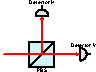
\includegraphics[width=0.7\columnwidth]{figures/QRNG.pdf}
	\caption{A simple implementation of a quantum random number generator. A single photon source is filtered to yield a stream of photons with $45^\circ$ diagonal polarisation. These pass through a polarising beamsplitter, which transmits vertically polarised photons and reflects horizontally polarised ones. The diagonally polarised photons have 50/50 likelihood of triggering each of the detectors, yielding a binary stream of random bits.} \label{fig:QRNG}
\end{figure}

\subsection{Quantum key distribution (QKD)} \label{quantum-key-distribution-qkd}

??? hybrid with AES

In Sec.~\ref{one-time-pad-encryption} we introduced the one-time-pad cipher, the only provably (i.e information theoretically) secure classical encryption technique. However, despite its perfect security it was deemed highly impractical due to the need to continually establish new secret keys because they can't be reused.

Quantum key distribution (QKD) refers to a set of quantum protocols for securely sharing random bit-strings between parties. These could subsequently be used in any symmetric cipher, including the Holy Grail of the one-time-pad.

\subsubsection{BB84} \label{bb84}

The BB84 protocol (named after its inventors and the year of invention) \cite{bib:bb84} uses single photons to encode qubits used to share secret random bit-strings between end-users for use in a one-time-pad or other symmetric cipher (see Fig.~\ref{fig:BB84}).

We begin by defining two bases in which to encode a qubit with logical value 0 or 1 into the polarisation of a photon. The first is the horizontal/vertical basis:
\begin{align}
	|0\rangle &= |H\rangle,\nonumber\\
	|1\rangle &= |V\rangle.
\end{align}
The second is the diagonal/anti-diagonal basis (i.e a 45-degree polarization rotation compared to the first case): 
\begin{align}
	|0\rangle &= |D\rangle = \frac{1}{\sqrt{2}}(|H\rangle+|V\rangle),\nonumber\\
	|1\rangle &= |A\rangle = \frac{1}{\sqrt{2}}(|H\rangle-|V\rangle).
\end{align}
We now observe that if a qubit is measured in the same basis in which it is encoded we will necessarily recover the correct qubit value. If, on the other hand, we measure in the wrong basis, we get a random value (as per the quantum random number generator in Sec.~\ref{quantum-random-number-generation-qrng}).

Next Alice randomly chooses values to encode into her qubits (0 or 1), and also randomly chooses which bases to encode them in ($H$/$V$ or $D$/$A$). She sends a stream of such randomly encoded qubits to Bob. Bob now measures all the qubits in randomly chosen bases. The ones where by chance he measures in the basis Alice encoded in, they are guaranteed to share the result. If not, then not.

Alice then (publicly) announces which bases she encoded in, but not what the encoded values were (they are the secret). Bob similarly publicly announces which bases he measured in. They then filter their results to keep only the ones where encoding and measurement bases were consistent, from which they establish a shared random bit-string.

But how do we rule out a man-in-the-middle attack? To do this, Alice and Bob sacrifice some of their shared data and compare it over a public channel. If any inconsistencies are found it implies someone in the middle had intercepted those qubits, measured them, and re-encoded them, but not knowing which random basis to re-encode in, got it wrong. That is, because measurements collapse quantum states, intercept-resend attacks will introduce inconsistencies between the bit-strings of the end-users.

The final stage after sacrificing some shared bits to determine whether a man-in-the-middle attack has taken place is to perform \emph{privacy amplification}. The shared string may still may contain some exposed bits, which is mathematically reduced to a shorter shared string with higher security. This can be made asymptotically strong.

\begin{figure}[!htb]
	\centering
	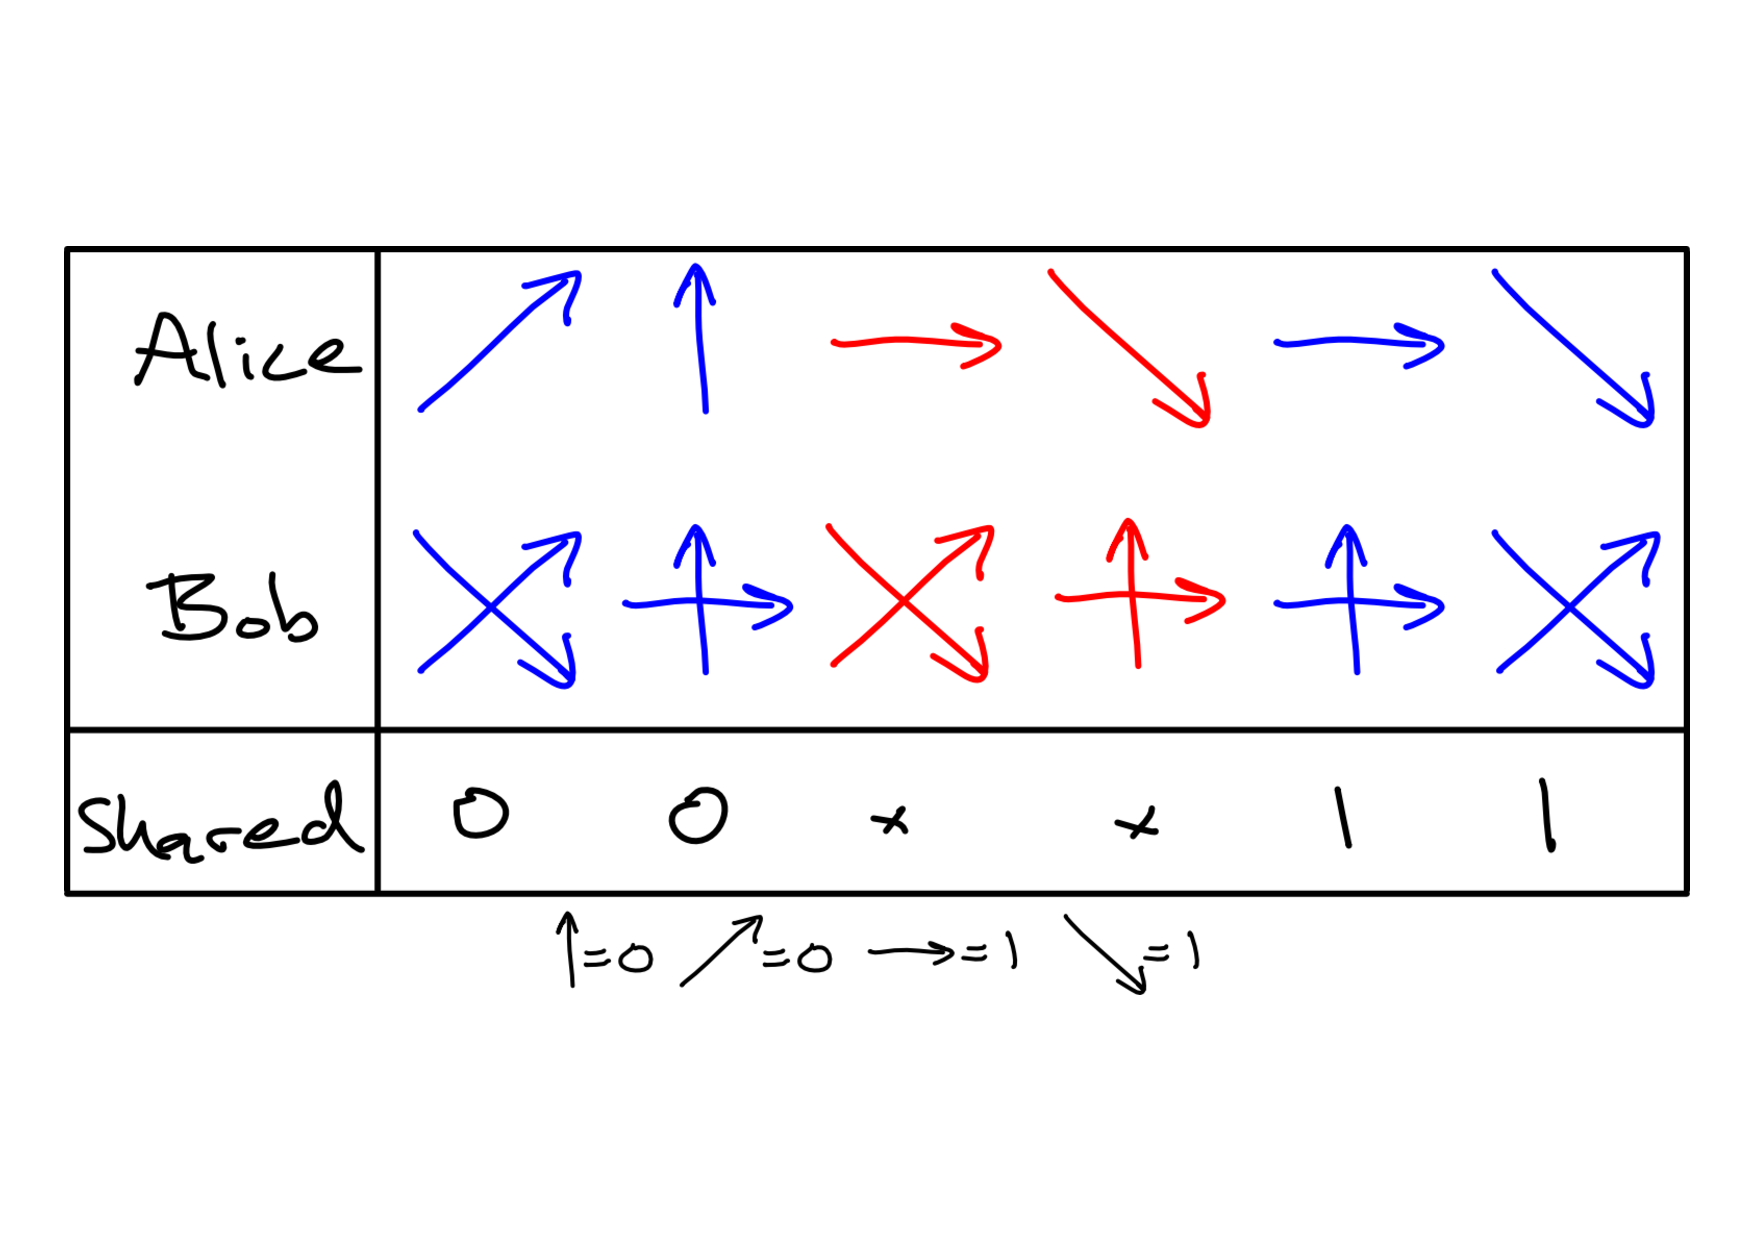
\includegraphics[width=\columnwidth]{figures/BB84}
	\caption{Example encodings and measurements for the BB84 protocol. Upon classical post-processing, Alice and Bob are left with secure, shared randomness that can be employed in a one-time-pad cipher for information-theoretically secure encryption.} \label{fig:BB84}
\end{figure}

\subsubsection{E91} \label{e91}

The so-called E91 protocol (again named after the inventor and year of invention) \cite{bib:ekert1991quantum} makes the same promise and has similar operation to BB84. The difference between BB84 and E91 is that BB84 relies on the communication of single qubits whereas E91 relies upon both parties sharing an entangled Bell pair.

A Bell pair is a maximally entangled, two-qubit state, which can equivalently be written as
\begin{align}
	|\Psi\rangle &= \frac{1}{\sqrt{2}}(|H,H\rangle+|V,V\rangle)\nonumber\\
	&= \frac{1}{\sqrt{2}}(|D,D\rangle+|A,A\rangle),
\end{align}
in the horizontal/vertical and diagonal/anti-diagonal bases respectively. 

With a large number of such shared pairs, for each pair, the operation proceeds similarly to BB84. Alice randomly measures either in the horizontal/vertical basis or diagonal/anti-diagonal basis, after which Bob's state will be identical to her measurement outcome if he measures in the same basis or completely random if he doesn't. Over an unsecured channel, they then compare their measurement \emph{bases} after which the ones where they measured consistently must have been the same. Should someone attempt to perform an intercept-resend attack this will randomise their results resulting in inconsistencies upon sacrificing a subset of their shared bits for comparison, as per BB84.

While the operation and outcome are almost identical, the key difference here is that communicating shared Bell pairs has some practical advantages over communicating single qubits as per BB84. Bell pairs can in principle be communicated over very long distances using quantum repeater networks, which utilise the concepts of entanglement swapping and entanglement purification to overcome the issue that the probability of a single qubit successfully traversing a lossy channel drops exponentially with distance, thereby imposing distance limitations. Quantum repeaters overcome this efficiency problem and could in principle be utilised over extremely long distances in the presence of loss. This is one of the key reasons why a future quantum internet \cite{bib:RohdeQI} will be entanglement-based rather than single-qubit communication-based. Entanglement-based QKD has been demonstrated via satellite over distances $\sim$1,500km (see Fig.~\ref{fig:satellite})

\begin{figure}[!htb]
	\centering
	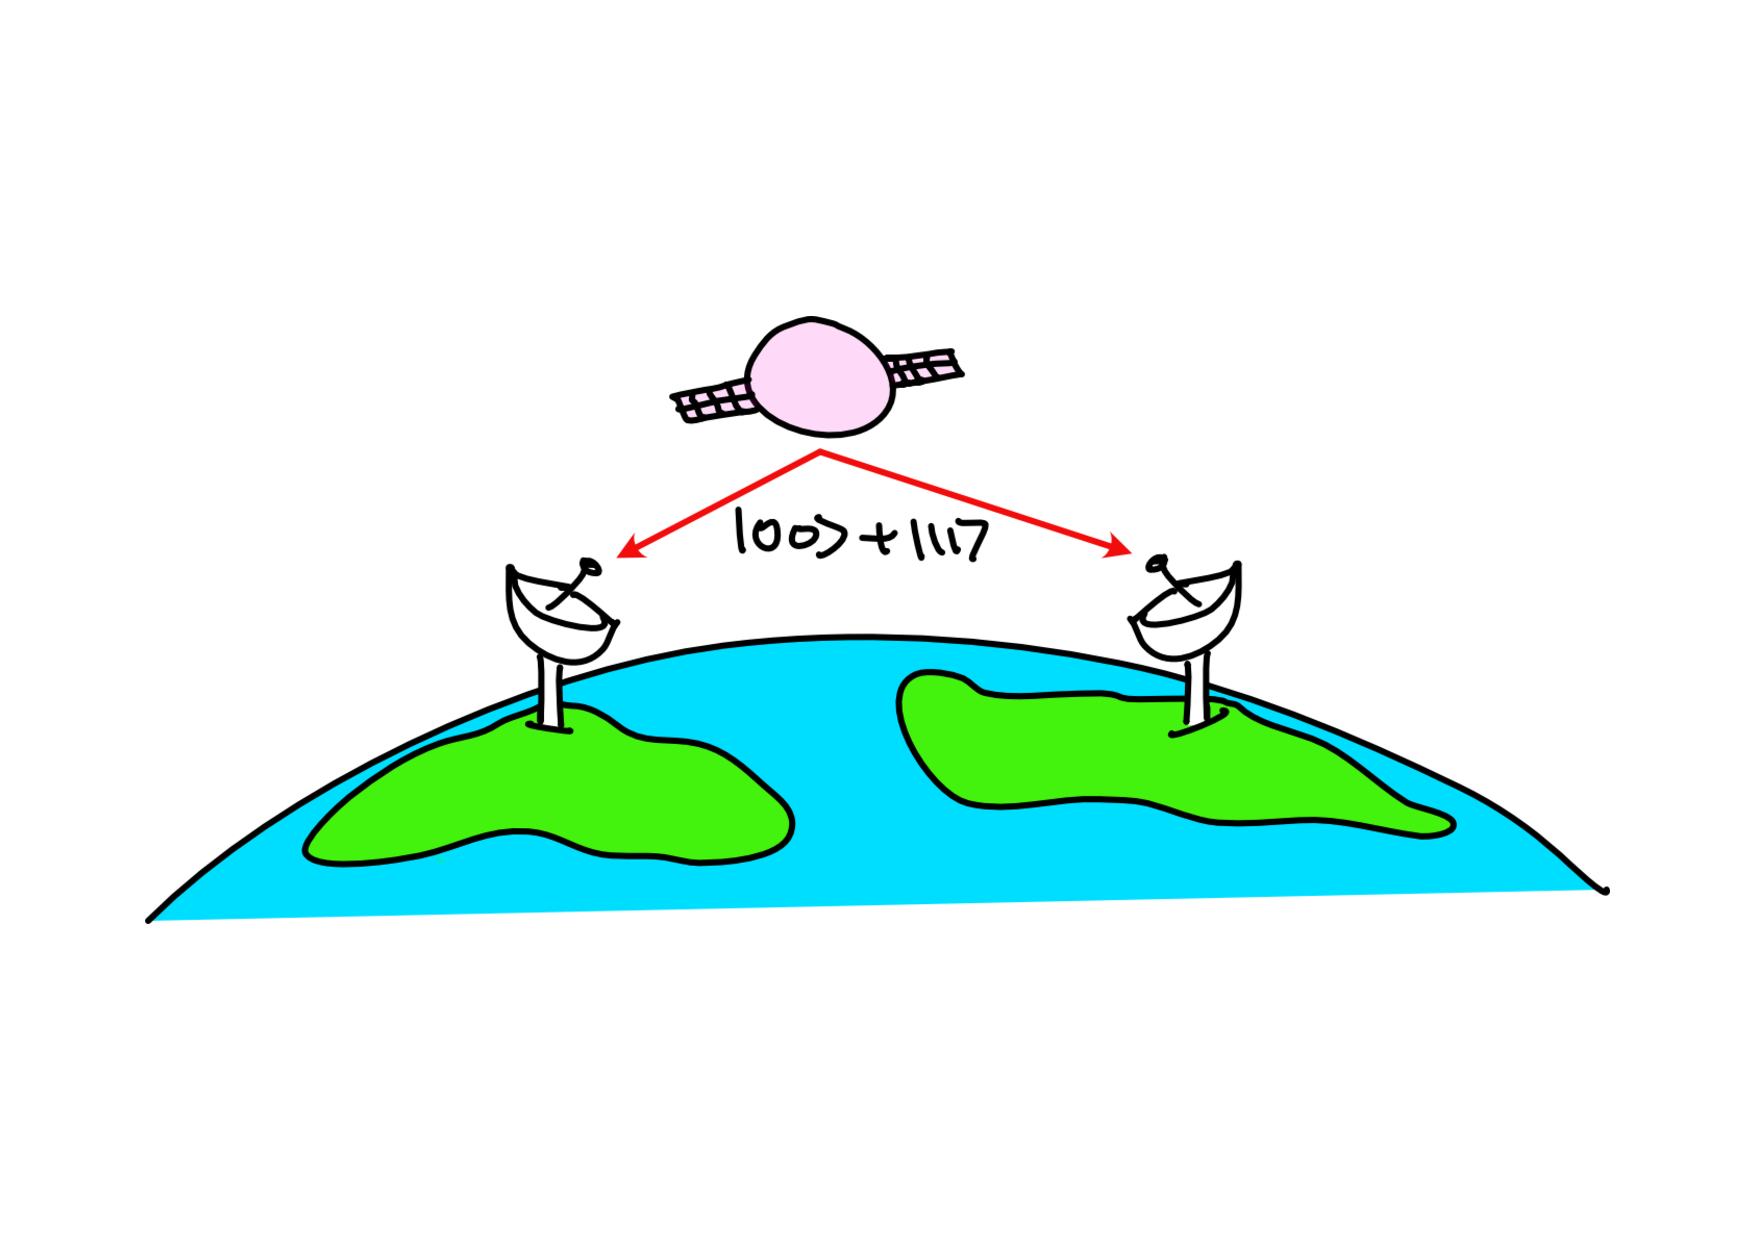
\includegraphics[width=\columnwidth]{figures/Satellite}
	\caption{Space-based entanglement distribution has successfully demonstrated low-bandwidth quantum key distribution over a range of $\sim$1,500km.} \label{fig:satellite}
\end{figure}

\subsubsection{Side-channel attacks} \label{side-channel-attacks-qkd}

While QKD is often quoted as offering \emph{perfect} security, this is far from the truth. QKD offers perfect security in the idealised theoretical setting whereby, in the case of E91 for example, two parties have shared Bell pairs and measure them. However, it is fanciful to think this ideal setting applies once the engineers get involved.

Bell pairs need to be prepared and it isn't as straightforward as it sounds to prepare a perfect Bell pair of the form,
\begin{align}
	|\Psi\rangle = \frac{1}{\sqrt{2}}(|H,H\rangle+|V,V\rangle),
\end{align}
that is exactly that, and nothing more, with no other entanglements or correlations with the environment or anything else. Should the prepared state deviate in any way from the ideal, this has the potential to open up avenues for information to be adversarially extracted. This might happen, for example, if the polarisation state were correlated with some other detectable photonic degree of freedom, or detectable signals emanating from the preparation device.

One type of attack that has previously undermined some QKD systems is the \emph{photon number splitting attack}. This exploits the fact that some photon sources sometimes produce multiple photons when they are only meant to produce one. Spontaneous parametric down-conversion (SPDC) sources, for example, exhibit this characteristic, as per the photon number distribution given in Eq.~\eqref{eq:SPDC_number}. Similarly, if single photon states are approximated using low intensity coherent states\footnote{Coherent states approximate laser light sources.} of the form,
\begin{align}
	\ket\alpha = e^{-\frac{|\alpha|^2}{2}} \sum_{n=0}^\infty \frac{\alpha^n}{\sqrt{n!}}\ket{n},
\end{align}
where $\alpha$ is the coherent amplitude, the photon number distribution is given by,
\begin{align}
	P(n) = e^{-\langle n\rangle}\frac{\langle n\rangle^n}{n!},	
\end{align}
where $\langle n\rangle=|\alpha|^2$ is the mean photon number. Note that higher-order photon-number terms always exists, irrespective of mean photon number $\langle n\rangle$. The likelihood of higher-order terms occurring is given by,
\begin{align}
	P(n>1) = \sum_{n=2}^\infty P(n).
\end{align}
For the case of mean photon number $\langle n\rangle=1$, this yields $P(n>1)\approx 0.264$. If those unwanted photons are correlated with the signal photon, intercepting them by tapping off part of the signal can reveal information to the adversary.

Another type of side-channel attack is \emph{timing attacks}. Consider the BB84 protocol where we randomly encode photonic qubits into different initial values $H$, $V$, $D$ or $A$. Suppose the setup was not perfectly temporally balanced and preparing some states caused them to exhibit a slight time offset compared to others. This could happen, for example, if encoding in different bases were implemented by following different optical paths to route through different polarisation rotation operations. This would effectively correlate the arrival time of photons with their polarisation encoding, whereby an eavesdropper could infer the polarisation state of photons from their detection time, enabling an undetectable intercept-resend attack. Although this particular attack can be mitigated by randomising state preparation times, it provides a conceptual example for just how easy it is for unwanted correlations introduced by imperfect engineering to thwart the in-principle perfect security offered by QKD.

This notion extends more generally to any other non-polarisation degree of freedom. If there exists distinguishing information between photons prepared into different basis states, measuring that degree of freedom reveals the associated polarisation state. Enormous care must be taken in real-world implementations to ensure that no such distinguishing information or unwanted correlations exist.

Similarly, sources, detectors and their control electronics may have detectable signatures of their own. Should an electronic control circuit emit distinct radiation signals upon different detection events taking place, this also provides avenues for side-channel attacks. There has been no shortage of tit-for-tat between QKD experimentalists demonstrating `perfect security' only for a simple exploit to later be discovered. In our minds, the vulnerabilities of QKD to side-channel attacks, which are not nearly as well studied as their classical counterparts, lead us to \emph{not} recommend relying exclusively on QKD for security, instead opting for hybrid approaches if QKD is to be employed (see Sec.~\ref{hybrid-cryptography}).

The other issue, as discussed previously, is that any secure connection requires channel authentication to eliminate eavesdroppers performing man-in-the-middle attacks, thereby making the security of systems only as strong as their channel authentication protocols. This requires either establishing a shared secret via direct means (e.g two spies meeting in person at the Embassy), relying on classical digital signatures, or on trusted third parties to act as guarantors.

\subsubsection{Denial-of-service (DoS) attacks} \label{denial-of-service-dos-attacks}

One very important attack vector especially relevant to QKD is denial-of-service (DoS) attacks. These are not intended to gather secret information, but to deny others the ability to securely communicate. Since QKD infrastructure will likely always be far more expensive and sparse than our classical networks, there will inevitably be less redundancy should links fail, making them far easier to disrupt. Additionally, due to the enormous precision and sensitivity of quantum systems, combined with the fact that broadcasting quantum messages is not possible, instead requiring point-to-point communication, such disruption is relatively easy compared to classical systems which are far more versatile and robust.

\subsection{Satellite-based QKD} \label{satellite-qkd}

China's satellite for entanglement distribution is one of the most impressive engineering achievements in our field in recent years, allowing Bell pairs to be shared across a distance of over 1,500km. The satellite contains a spontaneous parametric down-converter (SPDC) entanglement source, the most readily available type of entanglement source. Using this satellite Chinese researchers were able to demonstrate QKD over extremely long distances. It is worth commenting on the future prospects of this method of entanglement distribution.

The SPDC source produces states of the form,
\begin{align} \label{eq:SPDC}
	\ket\psi_\mathrm{SPDC} = \sqrt{1-\chi^2}\sum_{n=0}^\infty \chi^n \ket{n,n},
\end{align}
where $|\chi|<1$ characterises the pump power. That is, in the photon-number degree of freedom they exhibit a photon-number distribution of,
\begin{align} \label{eq:SPDC_number}
P(n) = (1-\chi^2)\chi^{2n},
\end{align}
following a power-law with mean photon number,
\begin{align}
	\langle n \rangle &= \sum_{n=0}^\infty P(n) \cdot n = \frac{\chi^2}{1-\chi^2}.
\end{align}
In a type-II configuration \cite{???} these photon-pairs are polarization-entangled, which for low pump-power $\chi\ll 1$ approximate a Bell pair,
\begin{align}
	\ket\psi_\mathrm{SPDC} = \frac{1}{\sqrt{2}}(\ket{H,V} + \ket{V,H}),
\end{align}
upon post-selection on detecting a single pair. The rate of single Bell-pair production using this technique is on the order of GHz.

The atmosphere introduces a loss rate of around 40dB at these frequencies, meaning that for both photons to reach the Earth the loss rate is around 80dB. That is, 1 in $10^8$ Bell pairs successfully reach the ground. This reduces our state preparation rate of GHz to a detection rate on the order of Hz. The 40dB of loss per channel is physically enforced. There isn't any foreseeable way to reduce atmospheric attenuation directly.

This is a rate far too slow to perform any real-time communication. To hold a phone call, for example, using a perfectly secure one-time-pad wouldn't be viable. Instead, a hybrid scheme would have to be employed whereby a short private key is shared for use in say AES-256, which can be reused and only requires 256 bits in advance. Thankfully AES is believed to be quantum-robust. Nonetheless, it undermines any claim of perfect information-theoretic security.

What can be done to overcome this? The options are limited, but the most obvious one is to employ multiplexing (e.g frequency, spatial or temporal) to boost bandwidth. This is harder than it sounds. To implement frequency multiplexing, for example, to achieve ground GHz bit-rates would require billions of independent sources operating at distinct frequencies. However, our lab SPDC sources tend to operate at specific frequencies and cannot be so easily be arbitrarily frequency-tuned.

The second major issue is that to achieve entanglement distribution beyond line of sight, multiple satellites would need to be employed, with some implementing entanglement swapping. For this to take place we need to know the exact time of arrival of different photons, so that entangling gates can be performed between them. However SPDC sources produce photons randomly, they are not so-called `push-button' sources that create photon pairs on demand.

Given the atmospheric loss rates, which can't readily be overcome, it is questionable whether space-based entanglement distribution is the way forward. Static ground-based networks are far simpler from an engineering perspective.

\subsection{Quantum repeaters \& trusted nodes} \label{quantum-repeaters-trusted-nodes}

Photonic entanglement distribution suffers some serious obstacles:
\begin{itemize}
	\item Single photons cannot be amplified to prevent loss. Their presence is binary, and once lost they are gone forever.
	\item When travelling through lossy mediums (e.g optical fibre or the atmosphere) loss is exponential with distance.
	\item When travelling through free space in vacuum (e.g between satellites) dispersion loss is quadratic with distance.
\end{itemize}
This may seem a devastating blow that effectively rules out long-range entanglement distribution altogether. Thankfully there are two avenues to overcoming this: trusted node networks, and quantum repeaters. The former is a bit of a cheat and doesn't promise perfect security, but has the advantage that we can readily do it today, while the latter is the ideal long-term goal, upholding the promise of robustness against man-in-the-middle attacks, but is far too difficult to implement on a meaningful scale using present-day technology.

\subsubsection{Quantum repeaters} \label{quantum-repeaters}

Quantum repeaters use a combination of entanglement swapping, purification and quantum memories to achieve long-range entanglement links that are robust against man-in-the-middle attacks \cite{bib:dur98}.

Entanglement swapping (see Fig.~\ref{fig:swapping}) allows an entangling measurement between two halves of two distinct Bell pairs to fuse them together into a single Bell pair with extended range \cite{bib:1993PhRvL.70.1895B}.

\begin{figure}[!htb]
	\centering
	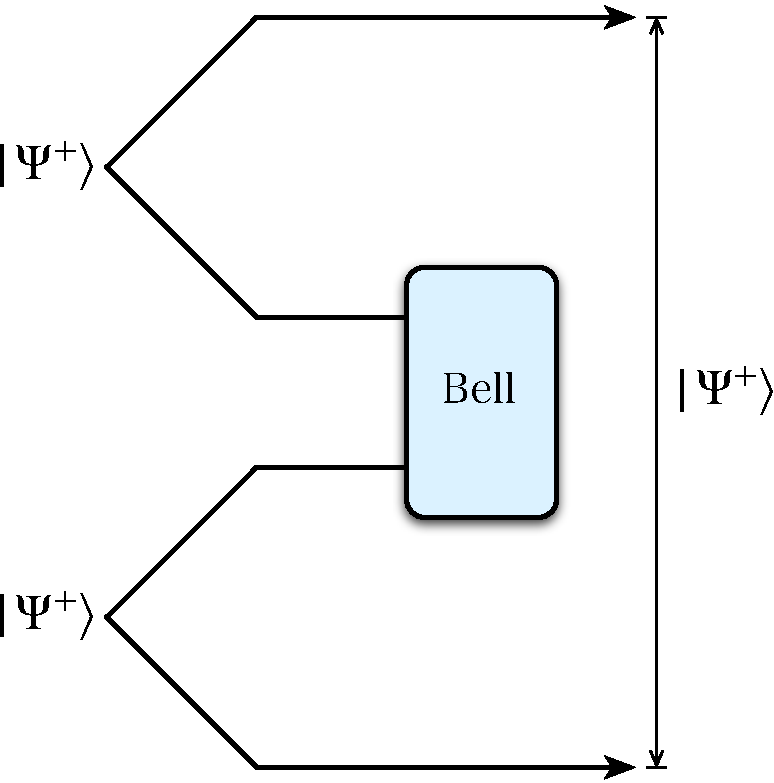
\includegraphics[width=0.7\columnwidth]{figures/Entanglement_swapping}
	\caption{Entanglement swapping takes two Bell pairs in series and performs a Bell measurement between one qubit from each pair. The resultant state is a longer-range Bell pair between the remaining two qubits.} \label{fig:swapping}
\end{figure}

Entanglement purification (see Fig.~\ref{fig:purification}) takes two noisy Bell pairs and transforms them into one less noisy Bell pair \cite{bib:Bennett96}. Specifically, for two Bell pairs of fidelity $F$, a standard purification circuit \cite{pan???} yields a single Bell pair with fidelity,
\begin{align}
F_\mathrm{out} = \frac{{F_\mathrm{in}}^2}{{F_\mathrm{in}}^2 + (1 - {F_\mathrm{in}})^2},
\end{align}
which has the property that so long as \mbox{$F_\mathrm{in}>1/2$}, the output fidelity is higher than the input fidelity, \mbox{$F_\mathrm{out}>F_\mathrm{in}$}, as per Fig.~\ref{fig:purification}(bottom).

\begin{figure}[!htb]
	\centering
	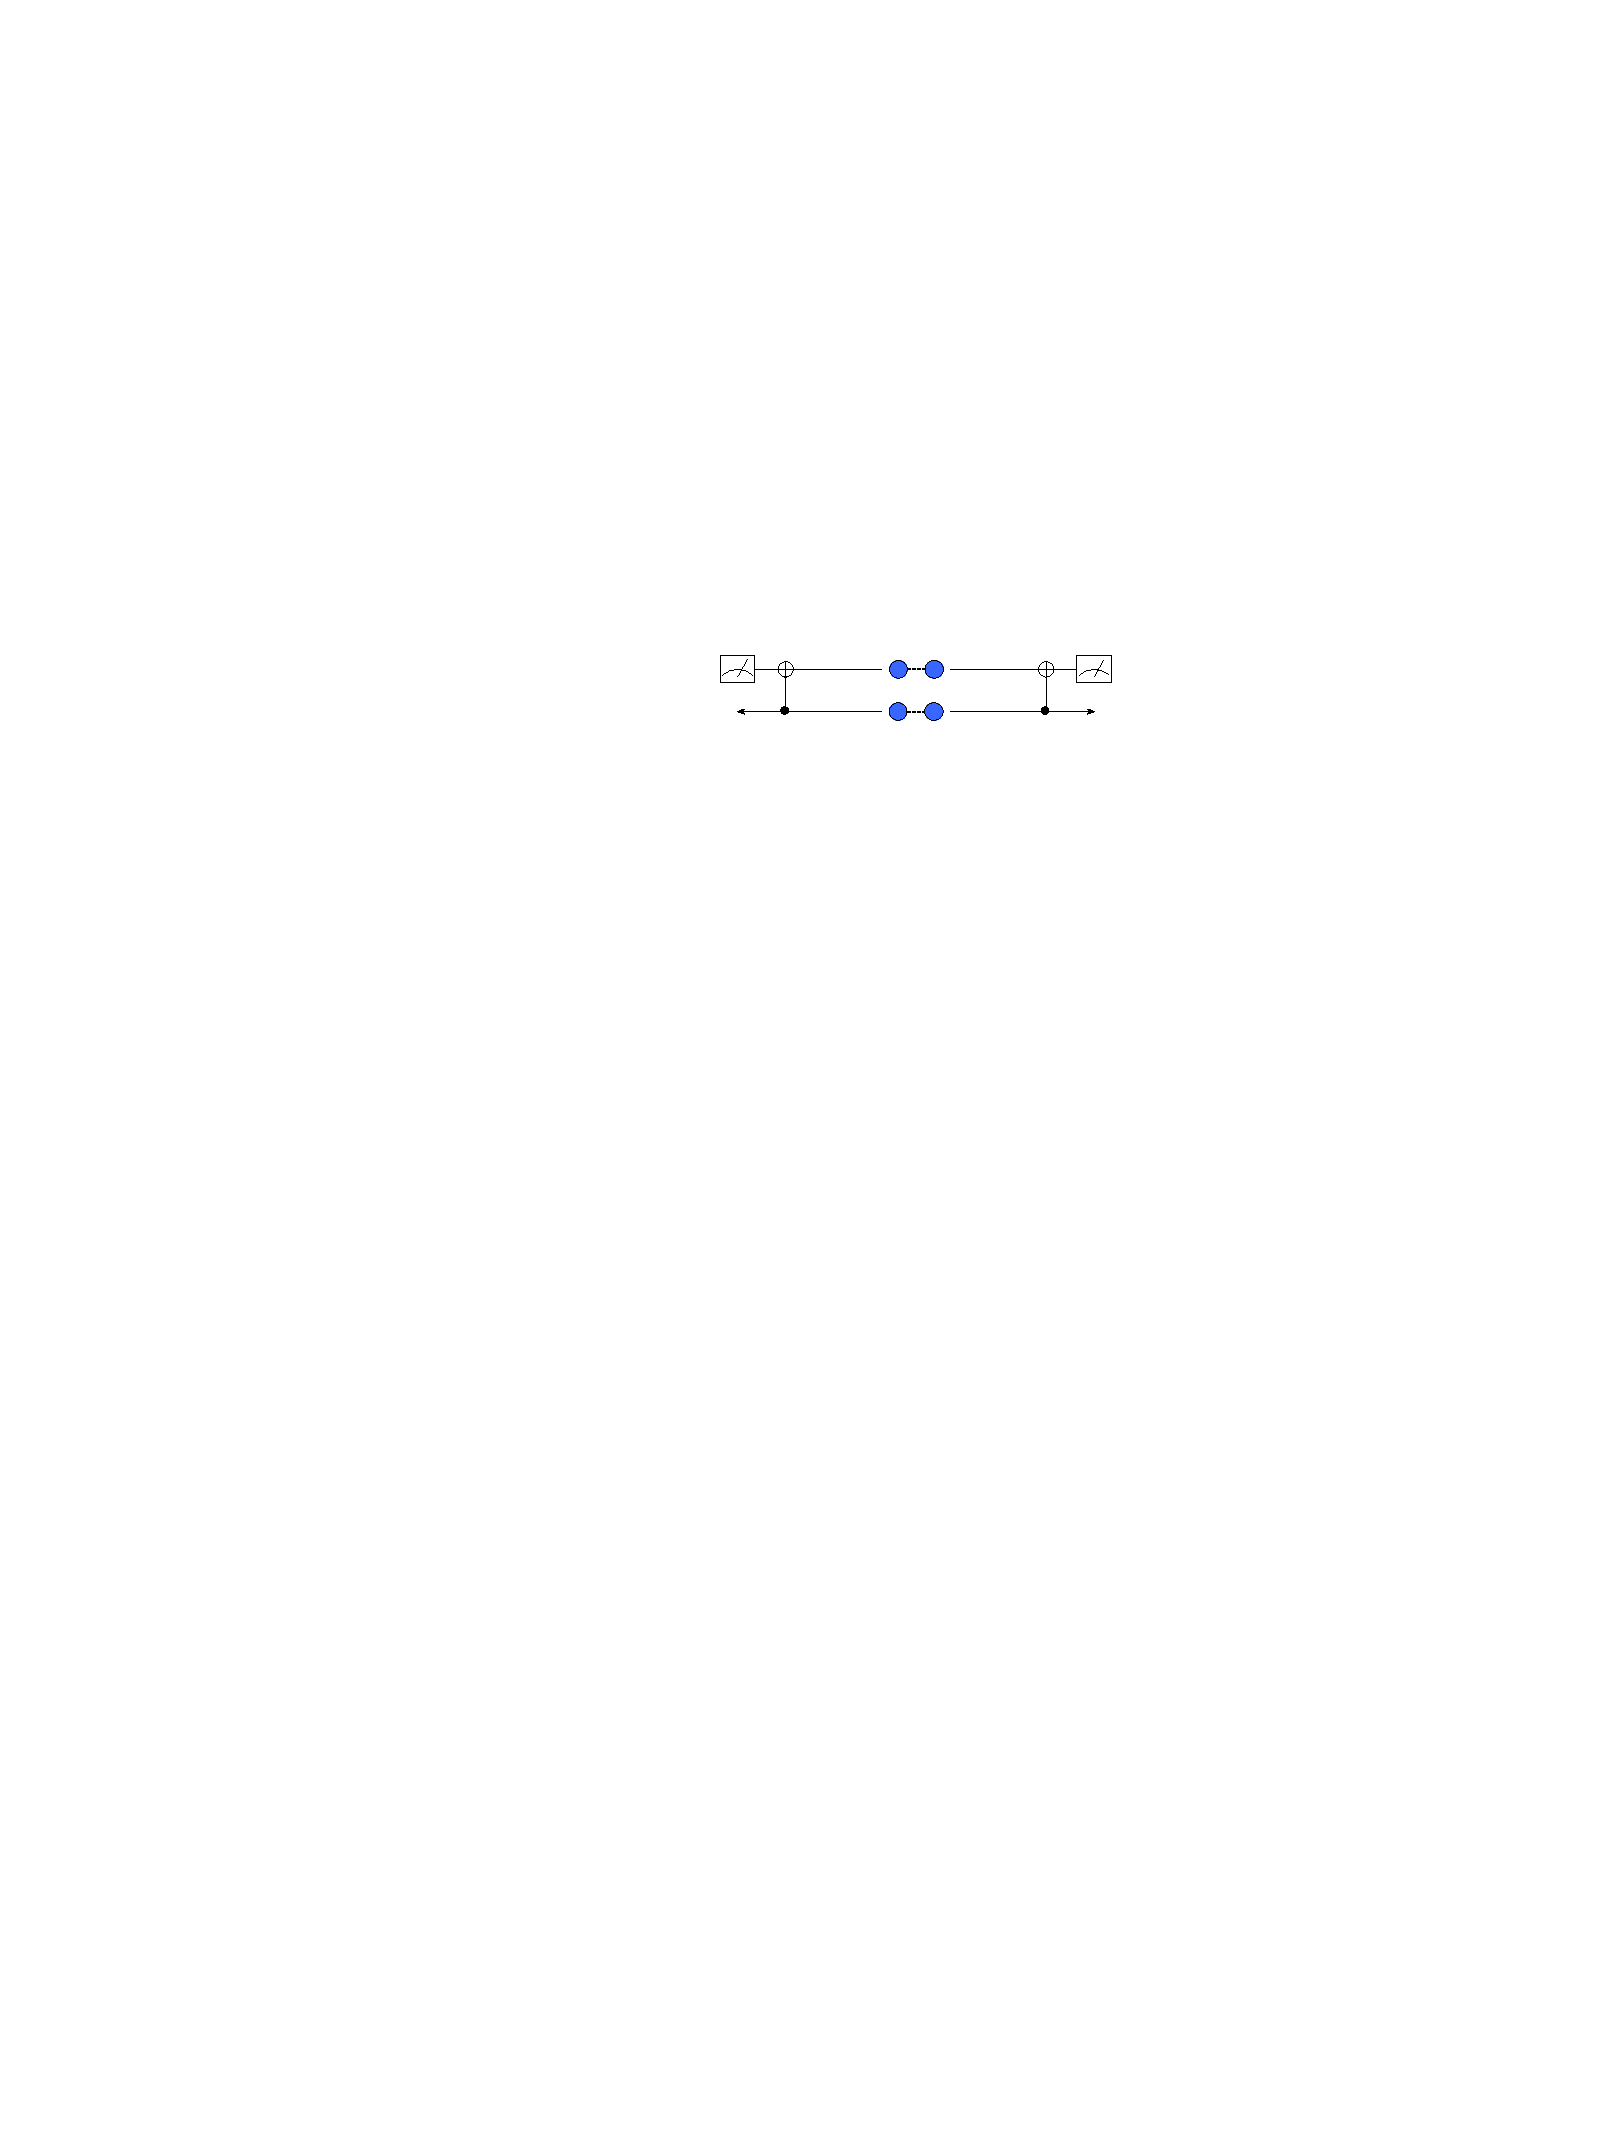
\includegraphics[width=\columnwidth]{figures/Entanglement_purification.pdf}\\
	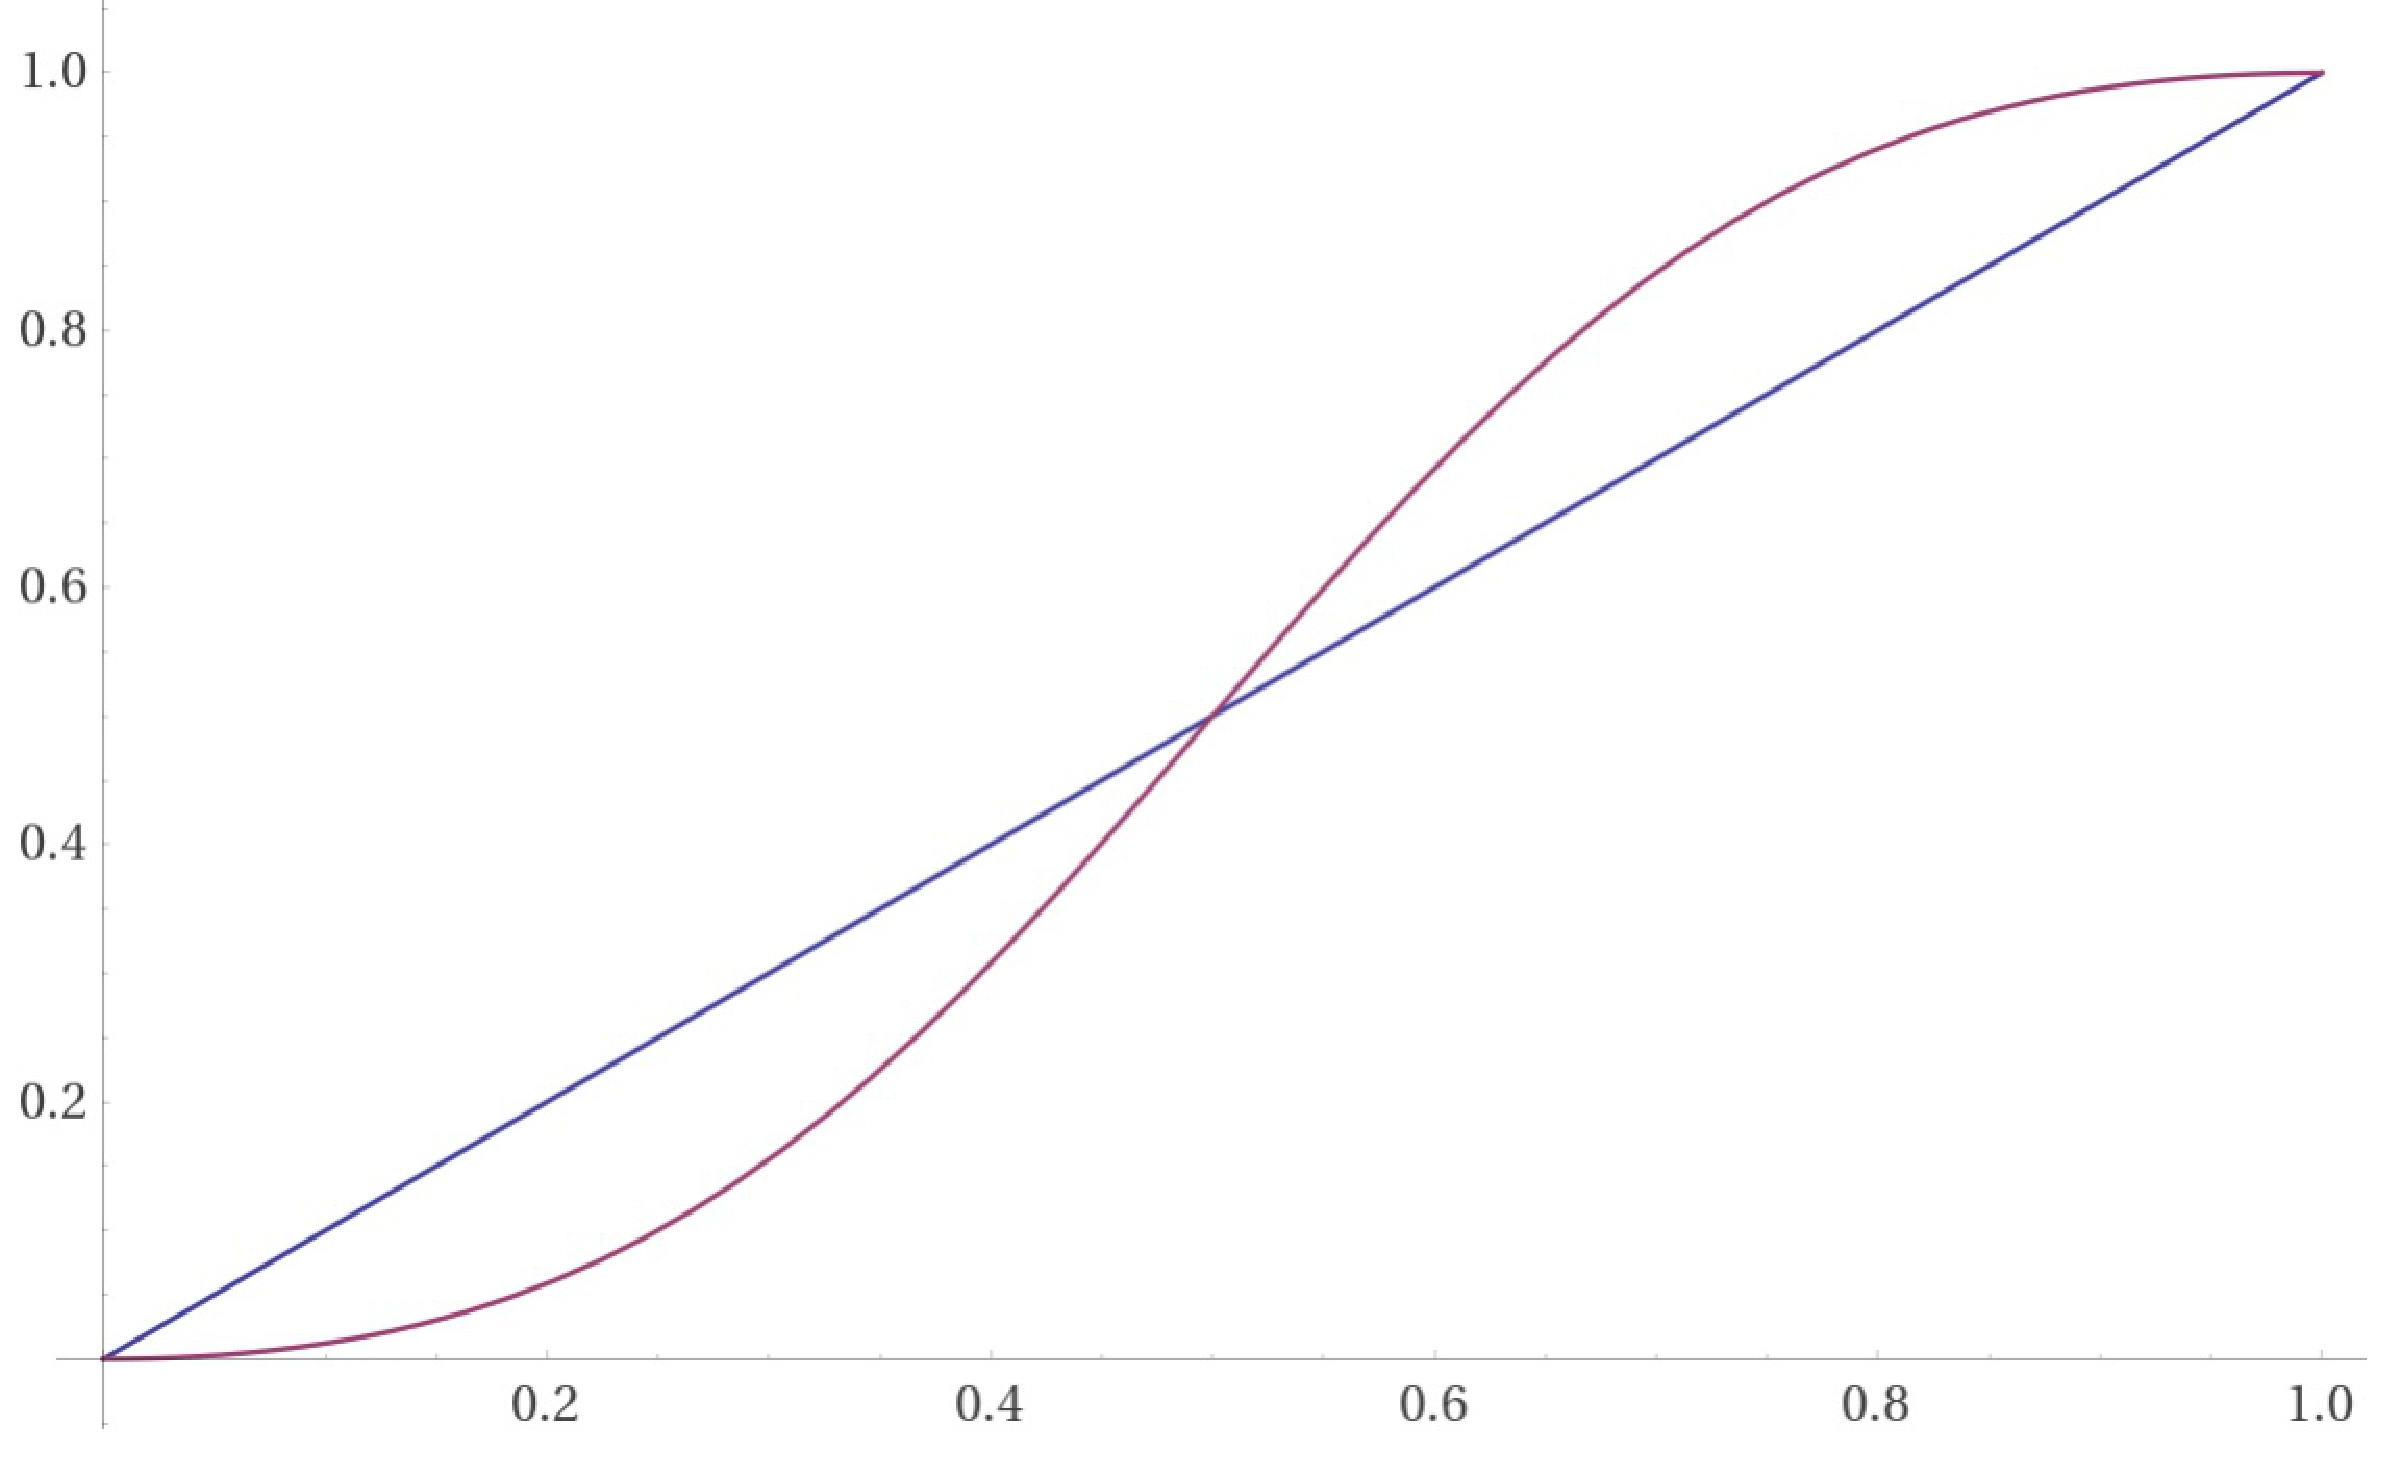
\includegraphics[width=\columnwidth]{figures/Purification_fidelity.pdf}
	\caption{(top) Entanglement purification takes two Bell pairs (shown in blue) and performs partial Bell measurements between corresponding qubits from each pair. The resultant state is a single Bell pair with higher fidelity than either of the originals. (bottom) Input/output relation for the fidelity of Bell pairs undergoing entanglement purification. The straight line acts as a visual guide for equality.} \label{fig:purification}
\end{figure}

Quantum repeaters subdivide our long-range link into shorter segments, interspersed with nodes that perform entanglement swapping to extend range and purification to improve quality (see Fig.~\ref{fig:repeater}).

\begin{figure*}[!htb]
	\centering
	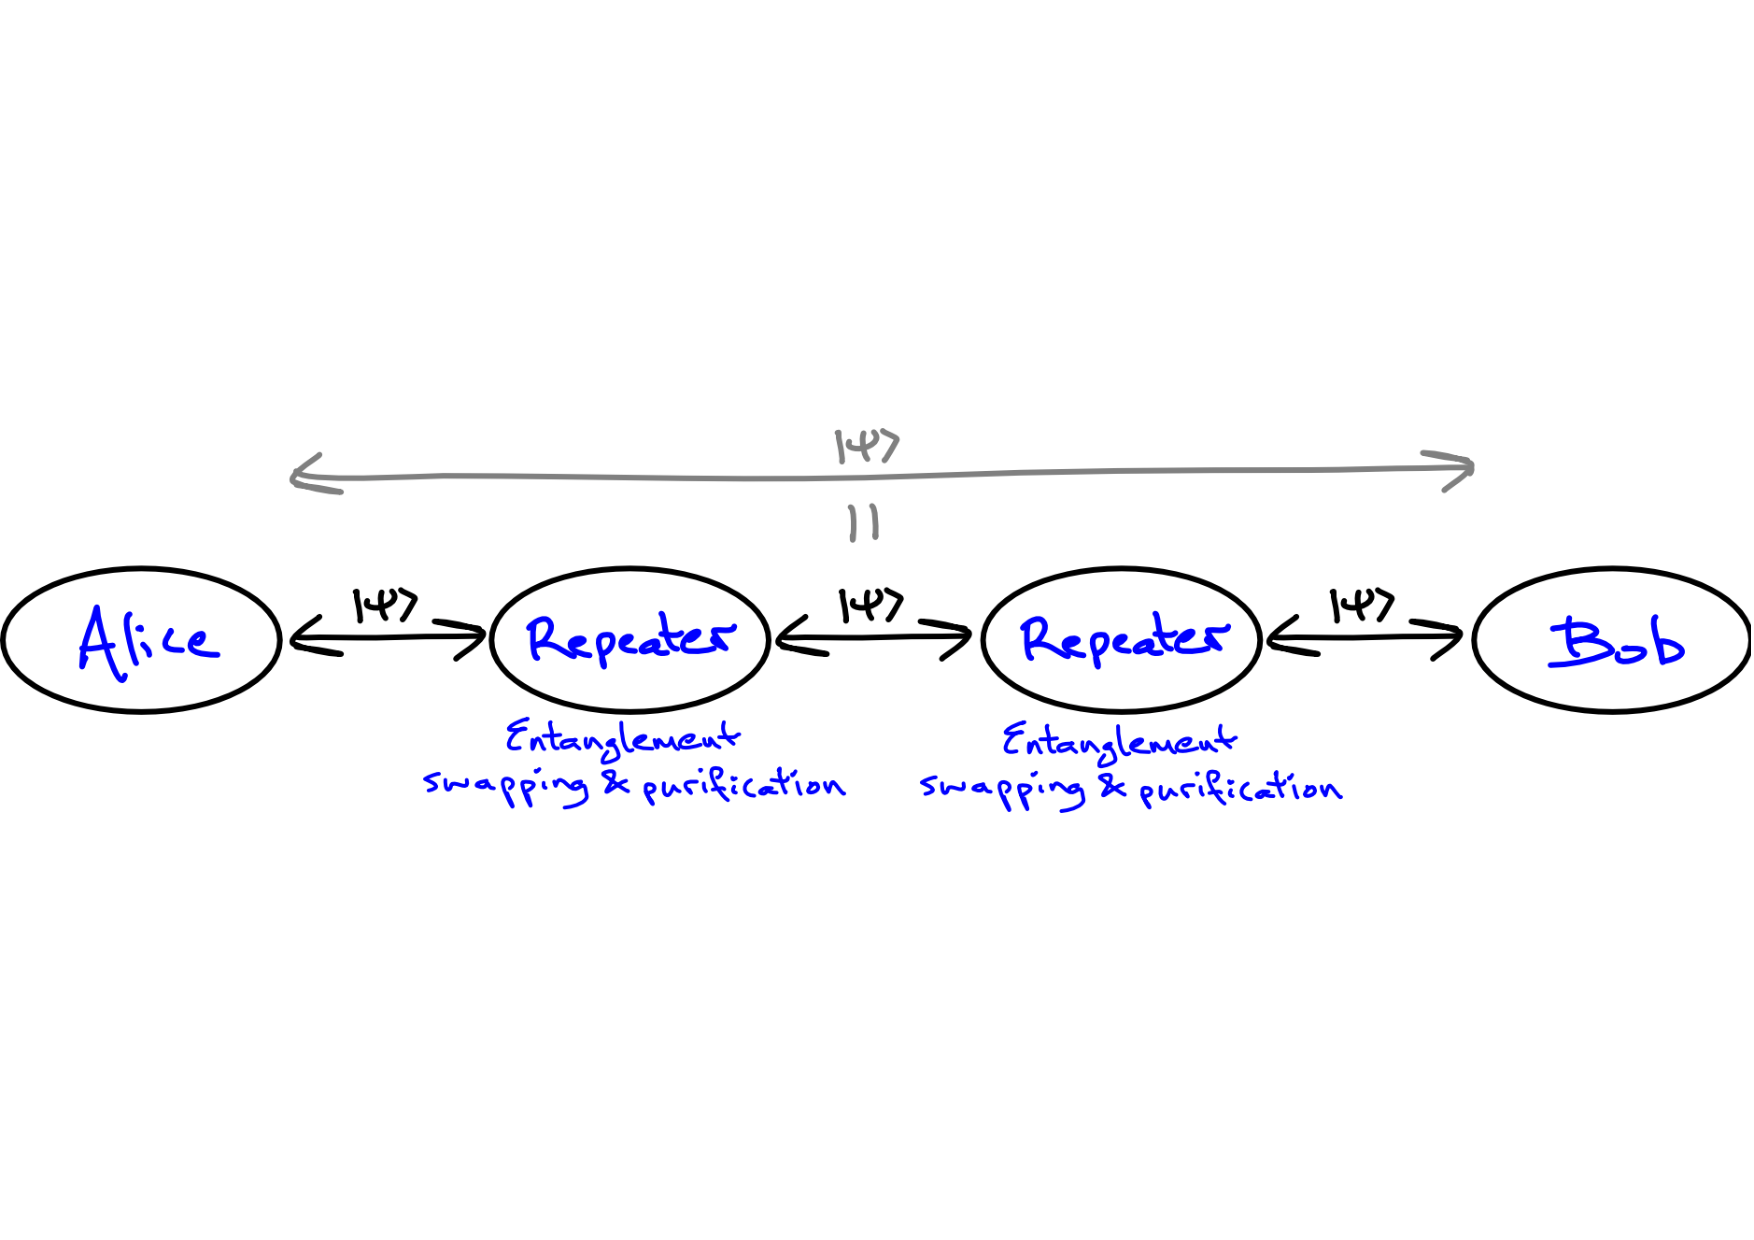
\includegraphics[width=2\columnwidth]{figures/Repeater}
	\caption{A quantum repeater network comprising entanglement links, entanglement swapping, and entanglement purification. Entanglement swapping extends the range of entanglement by `fusing' Bell pairs together, while entanglement purification takes multiple copies of noisy Bell pairs and reduced them down to one of higher quality. Quantum repeaters have the favourable property that efficiency only drops polynomially with distance, as opposed to the exponential decay expected from direct transmission.} \label{fig:repeater}
\end{figure*}

One might immediately question how this overcomes exponential loss. If all the individual segments need to work in the presence of loss, how is the effective loss rate any different to that of the entire length functioning at once? The key is that the individual segments don't need to succeed simultaneously. We employ a divide-and-conquer strategy, whereby we perform entanglement swapping pairwise, rather than all at once, creating slightly longer links. If they fail, we reattempt them. If they succeed, we go up a level and attempt joining the extended links. This necessarily requires high-efficiency, push-button quantum memories, something which is extremely challenging using present-day technology.

We can visualise an entanglement swapping network as a tree graph, where leaf nodes represent Bell pairs, and non-leaf nodes represent entanglement swapping operations. If we were to attempt to perform entanglement swapping in a linear fashion using a naive repeat-until-success strategy, repeatedly fusing on one extra link at a time, we could represent the tree diagram as per Fig.~\ref{fig:rep_linear}, where time flows from bottom to top.

\begin{figure}[!htb]
	\centering
	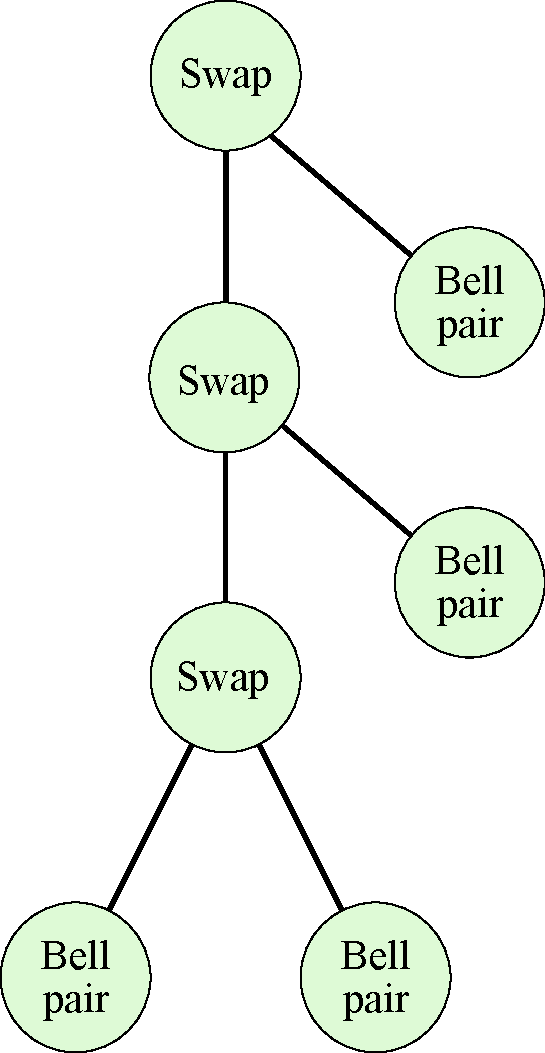
\includegraphics[width=0.5\columnwidth]{figures/Repeater_linear}
	\caption{Entanglement swapping hierarchy for a naïve in-series construction for a quantum repeater network. Time flows from bottom to top. With all swapping operations proceeding in series. This configuration is inefficient and not scalable.} \label{fig:rep_linear}
\end{figure}

Here the depth of the tree represents how many entanglement swapping operations must succeed in series for an overall success, which is linear in the number of Bell pairs and nodes. Any failures as a result of loss or non-deterministic operations whilst progressing up the tree requires us to recommence from the bottom of the tree since failure destroys the state. So the overall success rate drops exponentially with the number of nodes and we see that subdividing the length of the channel into segments achieves nothing in terms of efficiency.

The divide-and-conquer strategy behaves very different on the other hand. We can visualise this as a binary tree graph, as per Fig.~\ref{fig:rep_tree}.

\begin{figure}[!htb]
	\centering
	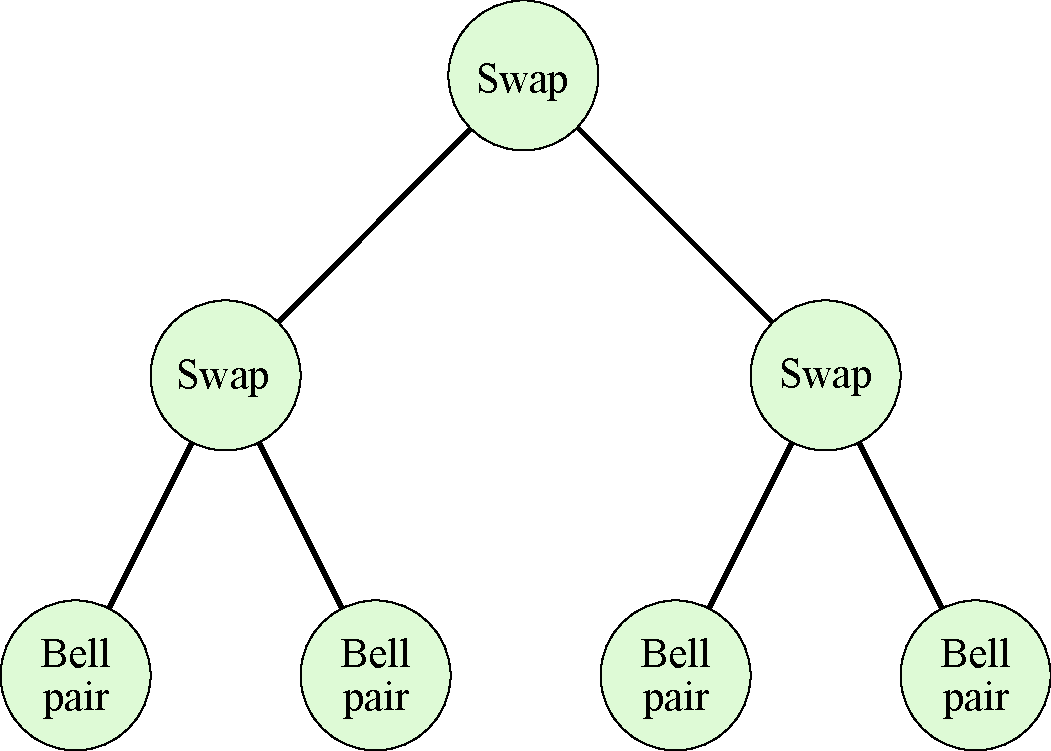
\includegraphics[width=\columnwidth]{figures/Repeater_tree}
	\caption{Entanglement swapping hierarchy for a divide-and-conquer based quantum repeater network. Time flows from bottom to top. Operations proceeding vertically up the graph take place in series, whereas different branches may be performed in parallel. If an operation fails, everything underneath it in the tree must be reattempted. This configuration allows efficient scaling in long-range networks.} \label{fig:rep_tree}
\end{figure}

Going sideways across the tree, things can be performed in parallel. Going upward through the tree they have to succeed in series, as before. When a SWAP operation fails, everything beneath it needs to be repeated, but separate branches are unaffected and can be held in quantum memory should a neighbouring branch need to be reattempted. Note that a binary tree has only logarithmic depth in the number of leaf nodes. The success probability drops exponentially with the depth of the tree, which is logarithmic, resulting in an overall polynomial scaling.

Let $N_i$ be the number of Bell pairs consumed to generate a Bell pair at level $i$ in the tree. Since a swapping operation requires two Bell pairs from the level below, we can write the recursive relationship,
\begin{align}
	N_{n+1} = \frac{2N_n}{p},
\end{align}
where $p$ is the success probability, incorporating loss and device non-determinism. This recursive relationship has the solution,
\begin{align}
	N_n &= L^{\log_2(2/p)} = \mathrm{poly}(L),
\end{align}where there are $L=2^n$ Bell pair segments at the lowest level of the $n$-level hierarchy. The effective efficiency is the inverse of this,
\begin{align}
	\eta = \frac{1}{N_n} = \mathrm{poly}^{-1}(L).
\end{align}

We now have an overhead in creating long-range entanglement with net efficiency scaling only inverse polynomially with distance. In principle, this makes the scheme `efficient' (in the computer science sense) over arbitrary distances. However, the engineering requirements for quantum repeaters are immense, requiring:
\begin{itemize}
	\item Entanglement swapping: to extend range.
	\item Entanglement purification: to improve quality.
	\item Quantum memories: to hold qubits while waiting upon others for further swapping or purification.
\end{itemize}

Each of these ingredients has strict mode-matching requirements to ensure photon indistinguishability, they must all be optimised to the same optical frequency, and must all be highly efficient. The last point is especially relevant to optical quantum memories, which typically suffer significant loss rates associated with input/output coupling and in-memory decay \cite{???}. Additionally, quantum memories must be `push button memories', whereby out-coupling is not random, but classically triggered.

While these individual ingredients have all been demonstrated in isolation, combining them into a long-range repeater network is beyond our current engineering capabilities.

\subsubsection{Trusted nodes} \label{trusted-nodes}

In a trusted node network (see Fig.~\ref{fig:trusted_node}) we again subdivide our long-range link into short segments over which loss rates and bandwidth are tolerable \cite{bib:salvail2010security}. Between each link is a \emph{trusted node}, whose job it is to be the recipient of the QKD key, retransmit it to the next trusted node, and destroy their copy of the key, thereby acting as a relay.

\begin{figure*}[!htb]
	\centering
	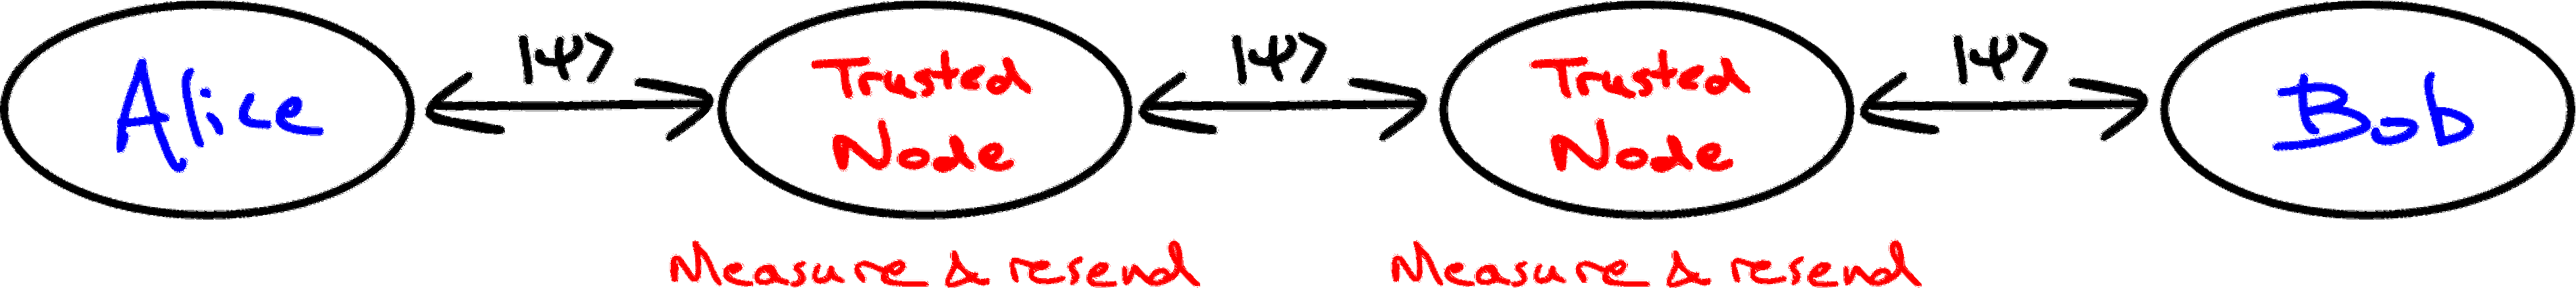
\includegraphics[width=2\columnwidth]{figures/Trusted_node}
	\caption{A trusted node network between Alice and Bob. The intermediate	nodes are necessary to overcome exponential loss against distance, but must be trusted to not compromise the key bits they measure and resend.} \label{fig:trusted_node}
\end{figure*}

Mathematically, the success rate of a link of length $L$ scales inverse exponentially as,
\begin{align}
	P(L) = e^{-\beta L},
\end{align}
where $\beta>0$ characterises loss per distance. If we subdivide the link length $L$ into $n$ segments, each segment will have length,
\begin{align}
	L_\mathrm{seg} = \frac{L}{n},
\end{align}
	with success rate,
\begin{align}
	P(L_\mathrm{seg}) = e^{-\beta L/n}.
\end{align}
With $n$ such links required to succeed in succession (not simultaneously), the overall success rate is,
\begin{align}
	P_\mathrm{net}(n) = \frac{P(L_\mathrm{seg})}{n} = \frac{P(L/n)}{n} = \frac{e^{-\beta L/n}}{n},
\end{align}
resulting in a trade-off from the exponential term into a linear term. In the large $n$ limit this scaling reduces to,
\begin{align}
	\lim_{n\to\infty} P_\mathrm{net}(n) = \frac{1}{n},
\end{align}
implying a linear number of repetitions are required to achieve success.

Although this type of intercept-resend strategy requires only linear time overhead in distance, its utility is limited to QKD as it does not distribute entanglement, only secret key bits. It suffers the obvious flaw that because it is based on intercept-resend --- also a type of attack --- the nodes must be absolutely secure, hence the name `trusted nodes'. If just a single node is compromised, so is the entire channel. The likelihood of the route being secure therefore drops exponentially with the number of trusted nodes --- we've effectively traded exponential photon loss for exponential security loss. Despite this limitation, for highly specialised purposes, such as point-to-point communication where all nodes are controlled by the same party, this provides security as good as the armed guards protecting them. This is the approach used in present-day long-range QKD links, most notably in China's extremely impressive national QKD network (see Fig.~\ref{fig:china_network}).

\begin{figure*}[!htb]
	\centering
	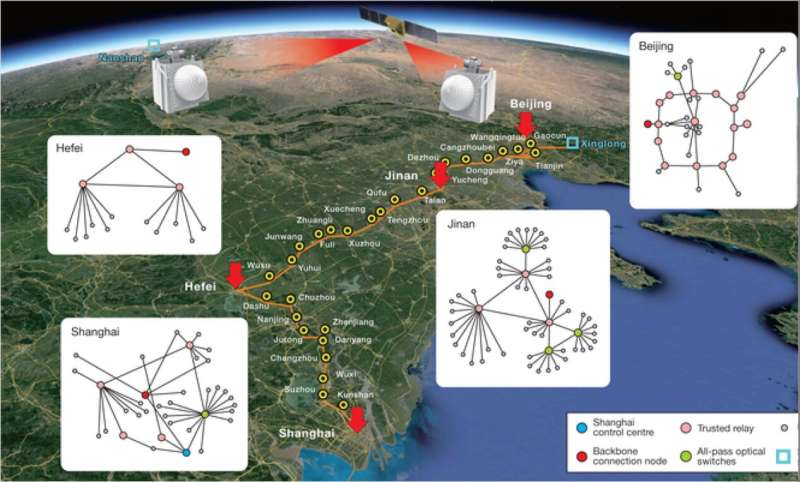
\includegraphics[width=2\columnwidth]{figures/China_network.jpeg}
	\caption{China's national quantum key distribution network, comprising a number of city-wide networks, a major backbone, and a long-range satellite. The network is based on trusted nodes as opposed to quantum repeaters. (Ask permission???)}	\label{fig:china_network} %???
\end{figure*}

\subsubsection{Multi-path QKD with trusted nodes}\label{multi-path-qkd-with-trusted-nodes}

Since a trusted node network requires that all nodes be secure, security drops exponentially with the number of trusted nodes --- if just one is compromised so is the key. This is a highly undesirable scaling characteristic, yet simultaneously appears the price to pay for relying on trusted nodes rather than quantum repeaters. This can however be improved upon without turning to quantum repeaters. The key, paradoxically, is to use \emph{more} nodes, but in parallel rather than in series.

We achieve this improvement by employing multiple routes through the network, each of which provides its own key. These keys are all combined to yield the master key (see Fig.~\ref{fig:multi_path}),
\begin{align}
	k_\textrm{master} = \bigoplus_i k_i.
\end{align}

The main observation here is that if multiple keys are independently routed, the master key is secure if \emph{any} of the constituent keys was secure. Equivalently, the key is only compromised if \emph{all} path keys $k_i$ are known. This achieves exponential scaling in the opposite direction --- security increases exponentially with the number of keys independently routed in parallel. We now have two exponentials: security decreases exponentially with the number of nodes in series and increases exponentially with the number of keys in parallel.

\begin{figure}[!htb]
	\centering
	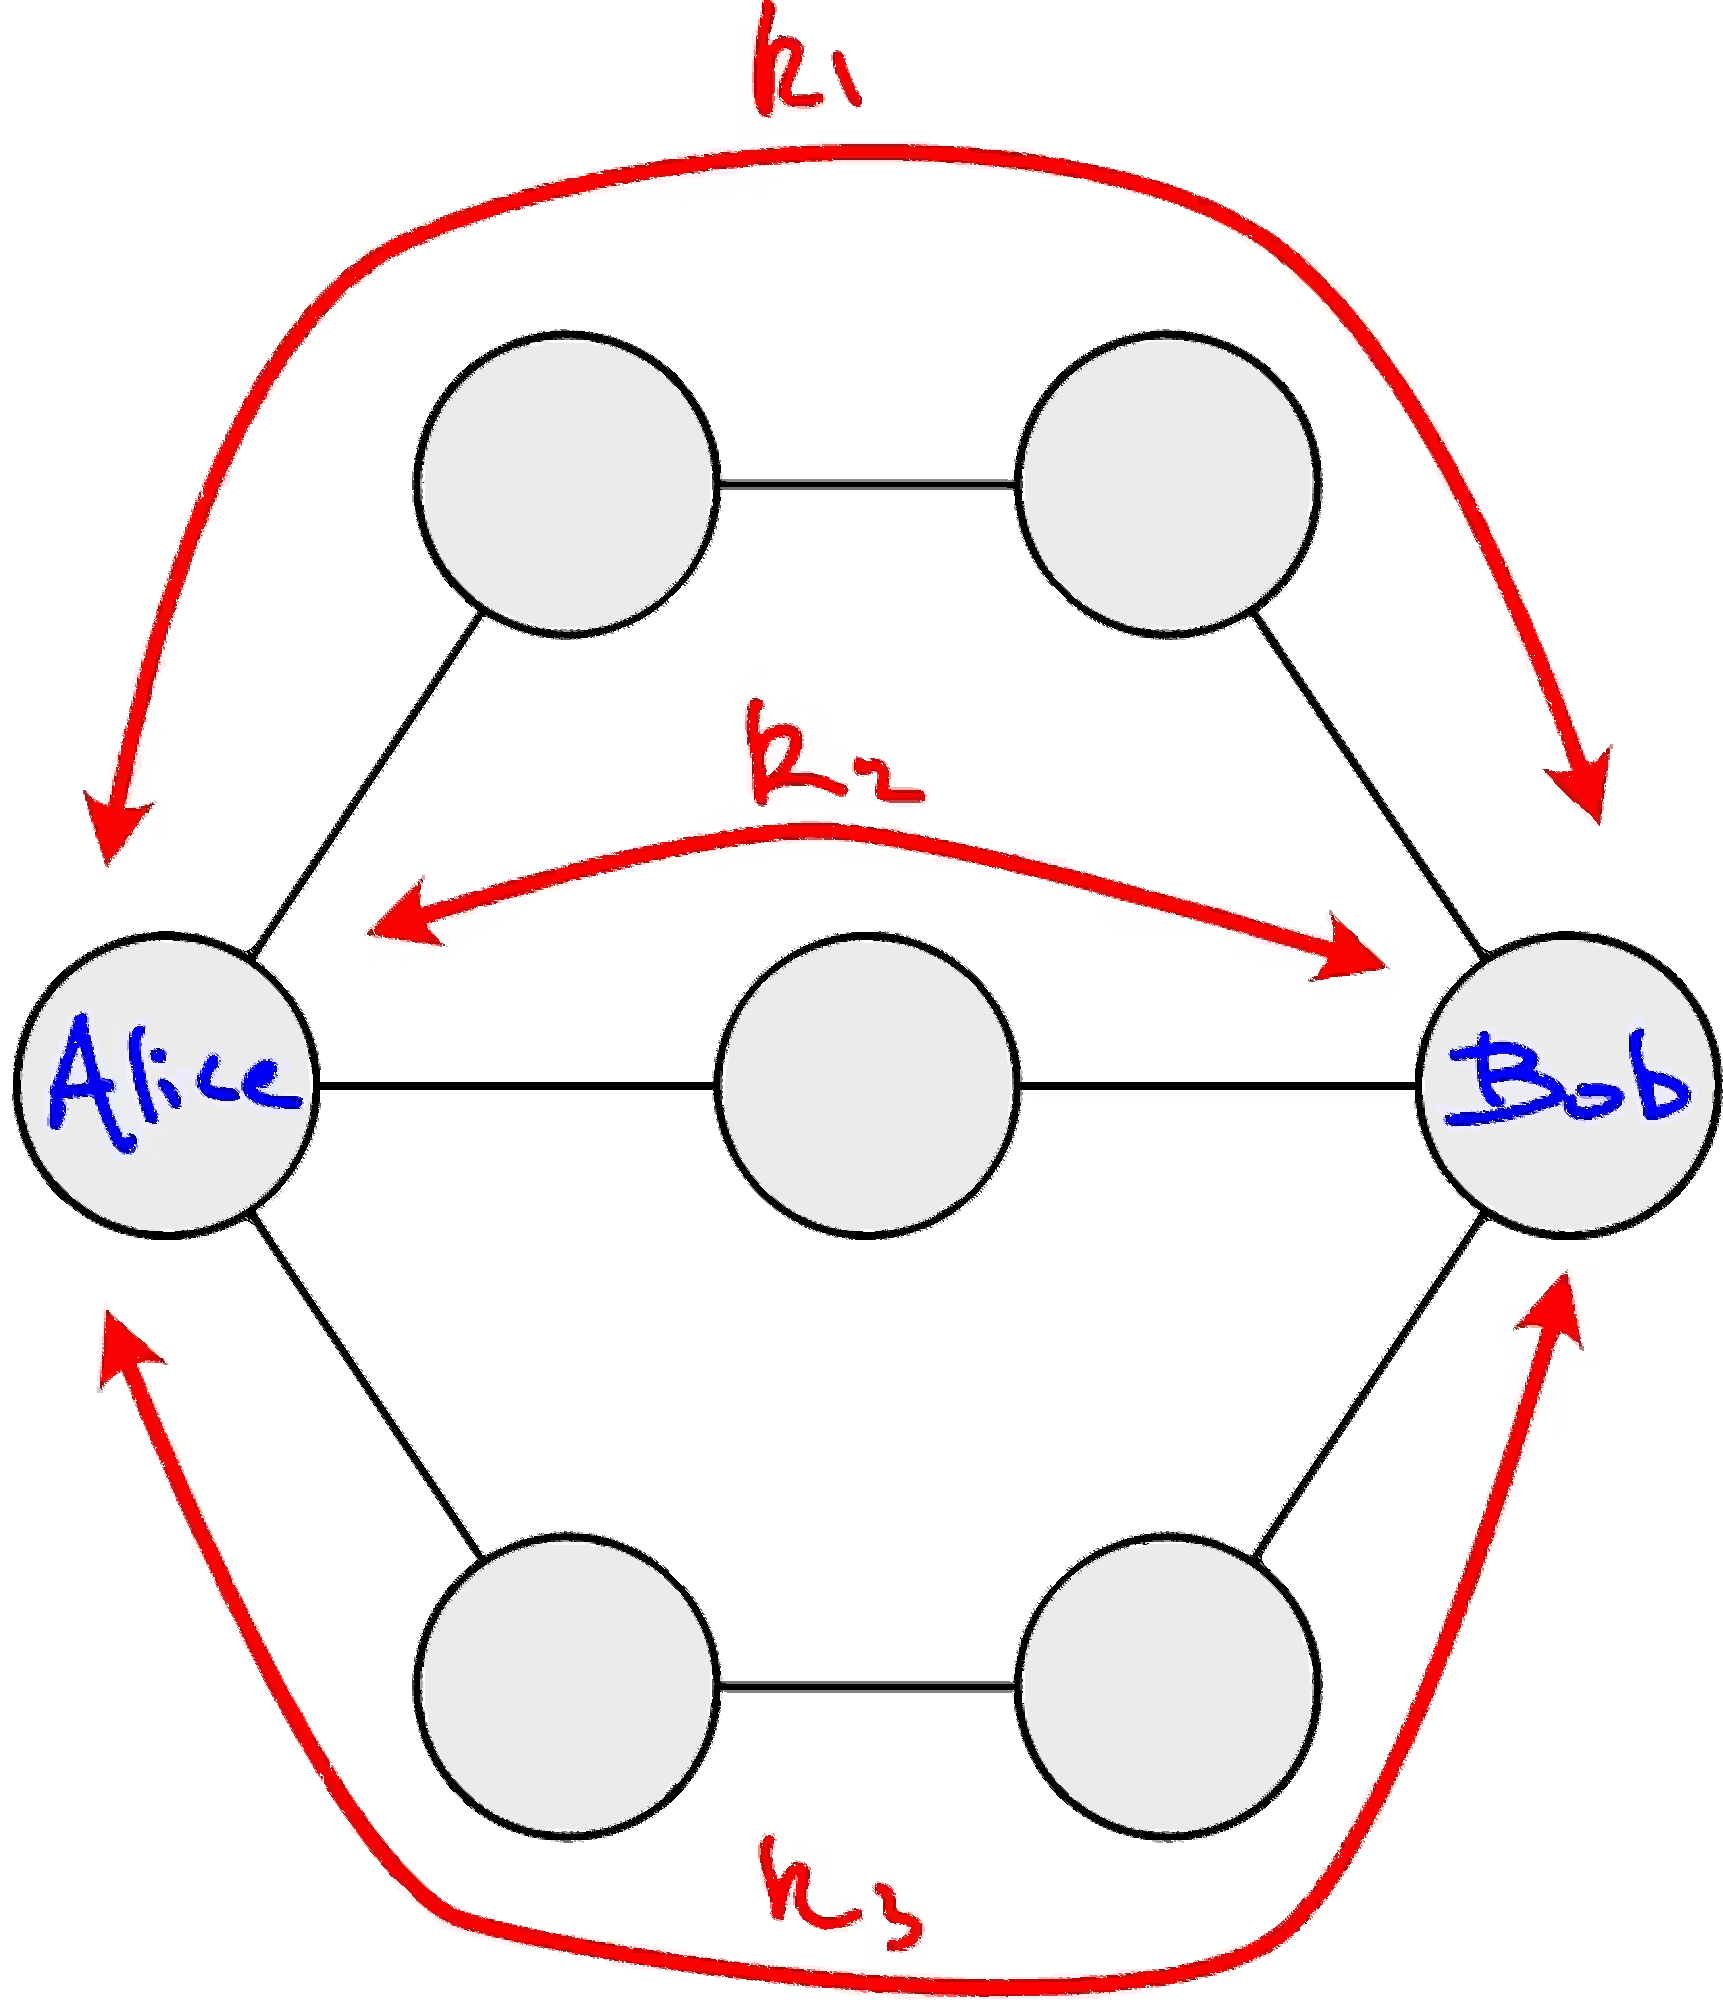
\includegraphics[width=0.6\columnwidth]{figures/Trusted_node_multipath}
	\caption{A multi-path trusted node QKD network. So long as there exists at least one path between Alice and Bob which is not compromised, a secure key may be established.} \label{fig:multi_path}
\end{figure}

We can easily derive a statistical model for the security of this network. Let $P(w_i)$ be the probability of node $i$ in path $w$ not being compromised. For a given path of length $L$, the path is secure if \emph{all} nodes are secure. Hence,
\begin{align}
	P_{\rm path}(w) = \prod_{i=1}^L P_{\rm node}(w_i).
\end{align}
For multiple paths, the key is secure if \emph{any} path is secure since all individual path keys $k_i$ must be compromised for $k_\mathrm{master}$ to be compromised. Thus for a set of $N$ vertex-independent paths through a network,
\begin{align}
	P_{\rm net}(\vec{w}) = 1-\prod_{i=1}^N [1-P_{\rm path}(w_i)].
\end{align}
If we make the simplifying assumption that all nodes have the same security $P_{\rm node}$ then a statistically independent model yields,
\begin{align}
	P_{\rm path}(L) &= {P_{\rm node}}^{L-2},\nonumber\\
	P_{\rm net}(N) &= 1-\prod_{i=1}^N (1-{P_{\rm node}}^{L_i-2}).
\end{align}
Making a further simplifying assumption that there are $N$ parallel paths all of length $L$, we obtain,
\begin{align}
	P_{\rm net} = 1-(1-{P_{\rm node}}^{L-2})^N.
\end{align}
Thus we see that individual paths have security that drops exponentially in their length, while the security of all paths jointly increases exponentially with the number of constituent paths. Importantly, for any value of $P_{\rm node}$, an appropriate choice of $N$ allows $P_{\rm net}$ to become arbitrarily close to 1.

\subsubsection{Channel authentication} \label{channel-authentication}

Although QKD in principle offers perfect security between two users, the robustness against man-in-the-middle attacks is based upon the assumption that those users know they are speaking to one another rather than an intermediary. This requires authentication via a classical channel. Ordinarily, we do this classically using digital signatures. However, our most popular current approaches for doing this (RSA \& ECC) are vulnerable to quantum attacks. To overcome this we can use one of two approaches:
\begin{itemize}
	\item Authentication using shared secrets, as discussed in Sec.~\ref{authentication-using-shared-secrets}.
	\item Authentication using post-quantum digital signatures, to be discussed in Sec.~\ref{post-quantum-cryptography-pqc}.
\end{itemize}
Both of these approaches are based on the security of hash functions, which we strongly believe to be robust against quantum attack vectors. In either case, some amount of data must be securely shared via other means, making QKD only as secure as whatever this alternate channel is. However, this shared secret is something that only needs to be shared once, and can be reused, unlike the one-time-pad key.

\subsection{Quantum anonymous broadcasting}

Quantum key distribution is a simple yet secure two-party cryptographic protocol. However, by employing multi-partite entanglement more elaborate cryptographic protocols can be constructed. One such protocol is \emph{quantum anonymous broadcasting} \cite{bib:QAB}, whereby users in a group are able to broadcast messages for all to hear, but such that the speaker's identity remains concealed.

To achieve this we rely on the distribution of multi-party GHZ states of the form
\begin{align}
	\ket\psi_\mathrm{GHZ}^{(N)} = \frac{1}{\sqrt{2}}(\ket{0}^{\otimes N} + \ket{1}^{\otimes N}),
\end{align}
where there are $N$ parties, each of whom receive one qubit from the collectively entangled state. GHZ states have the property that the action of a Pauli-$\hat{Z}$ gate on the state is independent of which qubit it is applied to,
\begin{align}
	\hat{Z}_i \ket\psi_\mathrm{GHZ}^{(N)} = \frac{1}{\sqrt{2}}(\ket{0}^{\otimes N} - \ket{1}^{\otimes N})\,\,\forall\, i.
\end{align}

If we let $m_i=\{0,1\}$ be the message of the $i$th user, then that user broadcasts their message by applying $\hat{Z}_i^{m_i}$ to their qubit, as per Fig.~\ref{fig:QAB}. If we impose the constraint that only one user speaks at a time, this has the effect of encoding $m_i$ into the phase of the GHZ state. Note that individual users always observe their reduced state to be the maximally mixed state, independent of $\vec m$,
\begin{align}
	\mathrm{tr}_{\bar i}(\hat{Z}_{j}^{m_j} \ket\psi_\mathrm{GHZ}^{(N)}\bra\psi_\mathrm{GHZ}^{(N)}\hat{Z}_{j}^{m_j}) = \frac{\hat{I_i}}{2}\,\,\forall\, i,j,
\end{align}
and are therefore unable to extract any information on their own.

\begin{figure}[!htb]
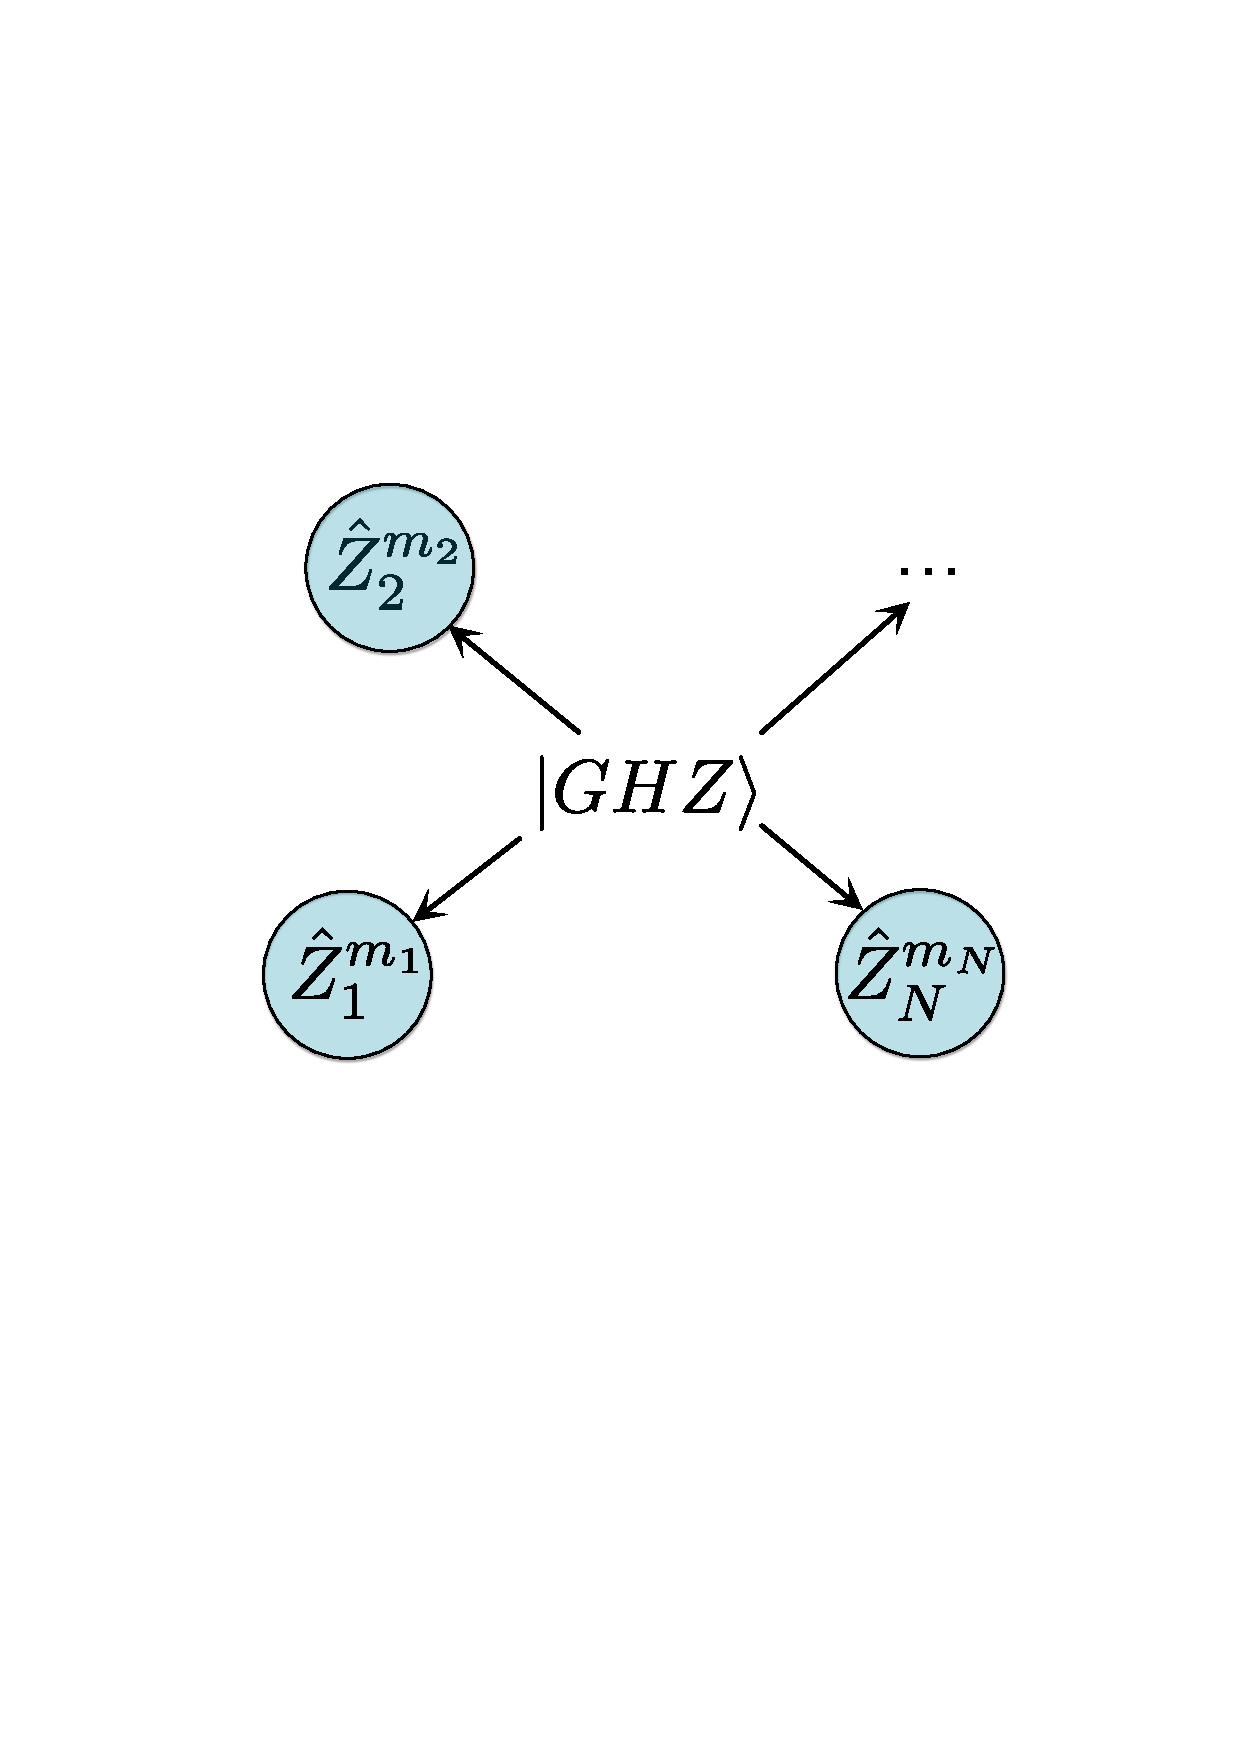
\includegraphics[width=0.6\columnwidth]{figures/QAB}
\caption{Quantum anonymous broadcasting protocol. The network distributes a $N$-qubit GHZ state between the $N$ users. User $i$ broadcasts their message by applying $\hat{Z}_i^{m_i}$ to their qubit. Subsequently, all users measure their qubits in the Pauli-$\hat{X}$ basis and publicly announce their results. The parity of all announced measurement results stipulates \mbox{$m=\bigoplus_{i=1}^N m_i$}. In the case where only one user broadcasts at a time, say user $i$, this reduces to $m_i$.} \label{fig:QAB}
\end{figure}

While the phase relationship in a GHZ state cannot be determined by any user, it can be determined collectively. If following the message broadcast all users measure their qubits in the Pauli-$\hat{X}$ basis (projecting onto \mbox{$\ket\pm = (\ket{0}\pm\ket{1})/\sqrt{2}$}), the parity of these collective measurement results stipulates the phase. Thus, following measurement all users publicly announce the outcome of their $\hat{X}$ measurements from which the phase, and hence message, becomes known to all.

It should be noted that while this simple protocol does offer information theoretic anonymisation of the speaker's identity, it suffers some significant limitations:
\begin{itemize}
\item Strictly only one user may broadcast at a time. If multiple users broadcast simultaneously, the reconstructed message will be given by the XOR of all broadcasters' messages,
	\begin{align}
		m = \bigoplus_{i=1}^{N} m_i.
	\end{align}
	This arises since message encoding is via the Pauli-$\hat{Z}$ operator, which accumulates modulo 2.
\item It is assumed all users are honest when announcing their measurement outcomes. A single dishonest user can disrupt the integrity of broadcast messages by dishonestly announcing random measurement outcomes. Thus, denial-of-service is trivial for anyone in possession of a qubit from the initially distributed GHZ state.
\end{itemize}

\subsection{Quantum anonymous voting}

The idea of using phase encoding to conceal identity can be generalised to \emph{quantum voting} \cite{bib:quantum_voting}, shown in Fig.~\ref{fig:quantum_voting}, where the goal is to implement a multi-party ballot such that users' individual voting decisions remain anonymised but their cumulative value can be collectively determined.

To do so we begin with a different type of entangled state, known as a \emph{ballot state},
\begin{align}
\ket{B} = \frac{1}{\sqrt{N+1}} \sum_{n=0}^N \ket{N-n}_T\otimes\ket{n}_V,
\end{align}
expressed in an occupation number representation, where $\ket{n}$ denotes an $n$-particle state, for example a photon-number state. This is a two-party state, where $V$ denotes the state held at the voting booth while $T$ is held by the tallyman.

Voters cast their votes sequentially, doing so by applying a \emph{voter operator} to the state held at the voting booth. The voter operator for the $i$th voter is defined via a phase-shift operator with angle $\delta_i$,
\begin{align}
\hat{v}_i = e^{i\hat{n}_V\delta_i},	
\end{align}
where $\hat{n}_V = \hat{a}^\dag_V\hat{a}_V$ is the (e.g photon-) number operator for mode $V$, and $\delta_i$ denotes the value of the $i$th voter's vote. 

The collective action of all voters is,
\begin{align}
\hat{v} &= \prod_{i=1}^{N_V} \hat{v}_i = e^{i\hat{n}\Delta}.
\end{align}
where,
\begin{align}
\Delta = \sum_{i=1}^{N_V} \delta_i,
\end{align}
is the cumulative vote.

When applied to the initial ballot state this yields,
\begin{align}
\ket{B'} = \frac{1}{\sqrt{N+1}} \sum_{n=0}^N e^{in\Delta} \ket{N-n}_T\otimes\ket{n}_V,
\end{align}
where the cumulative vote is encoded into the phases of the evolved ballot state.

Similar to quantum anonymous broadcasting, the voting booth and tallyman on their own observe the completely mixed reduced state,
\begin{align}
\mathrm{tr}_{V,T}(\ket{B'}\bra{B'}) &= \frac{1}{N+1} \sum_{n=0}^N \ket{n}_{T,V}\bra{n}_{T,V},
\end{align}
and are therefore unable to extract any information from it.

However, $\Delta$ can be extracted from the collective bipartite state $\ket{B'}$. Thus, the final stage is for the voting booth state to be reunited with the tallyman, who is now able to directly infer $\Delta$ using an appropriate measurement basis on $\ket{B'}$. Specifically, the tallyman measures the expectation value of the \emph{tally operator}, defined as,
\begin{align}
\hat{T} &= \sum_{n=0}^N n\ket{T_n}\bra{T_n},\nonumber\\
\hat{T}_n &= \frac{1}{\sqrt{N+1}} \sum_{k=0}^N e^\frac{2\pi ink}{N+1} \ket{N-k,k},
\end{align}
from which $\Delta$ is obtained via,
\begin{align}
\Delta = \frac{2\pi}{N+1}\bra{B'}\hat{T}\ket{B'}.
\end{align}

\begin{figure}[!htb]
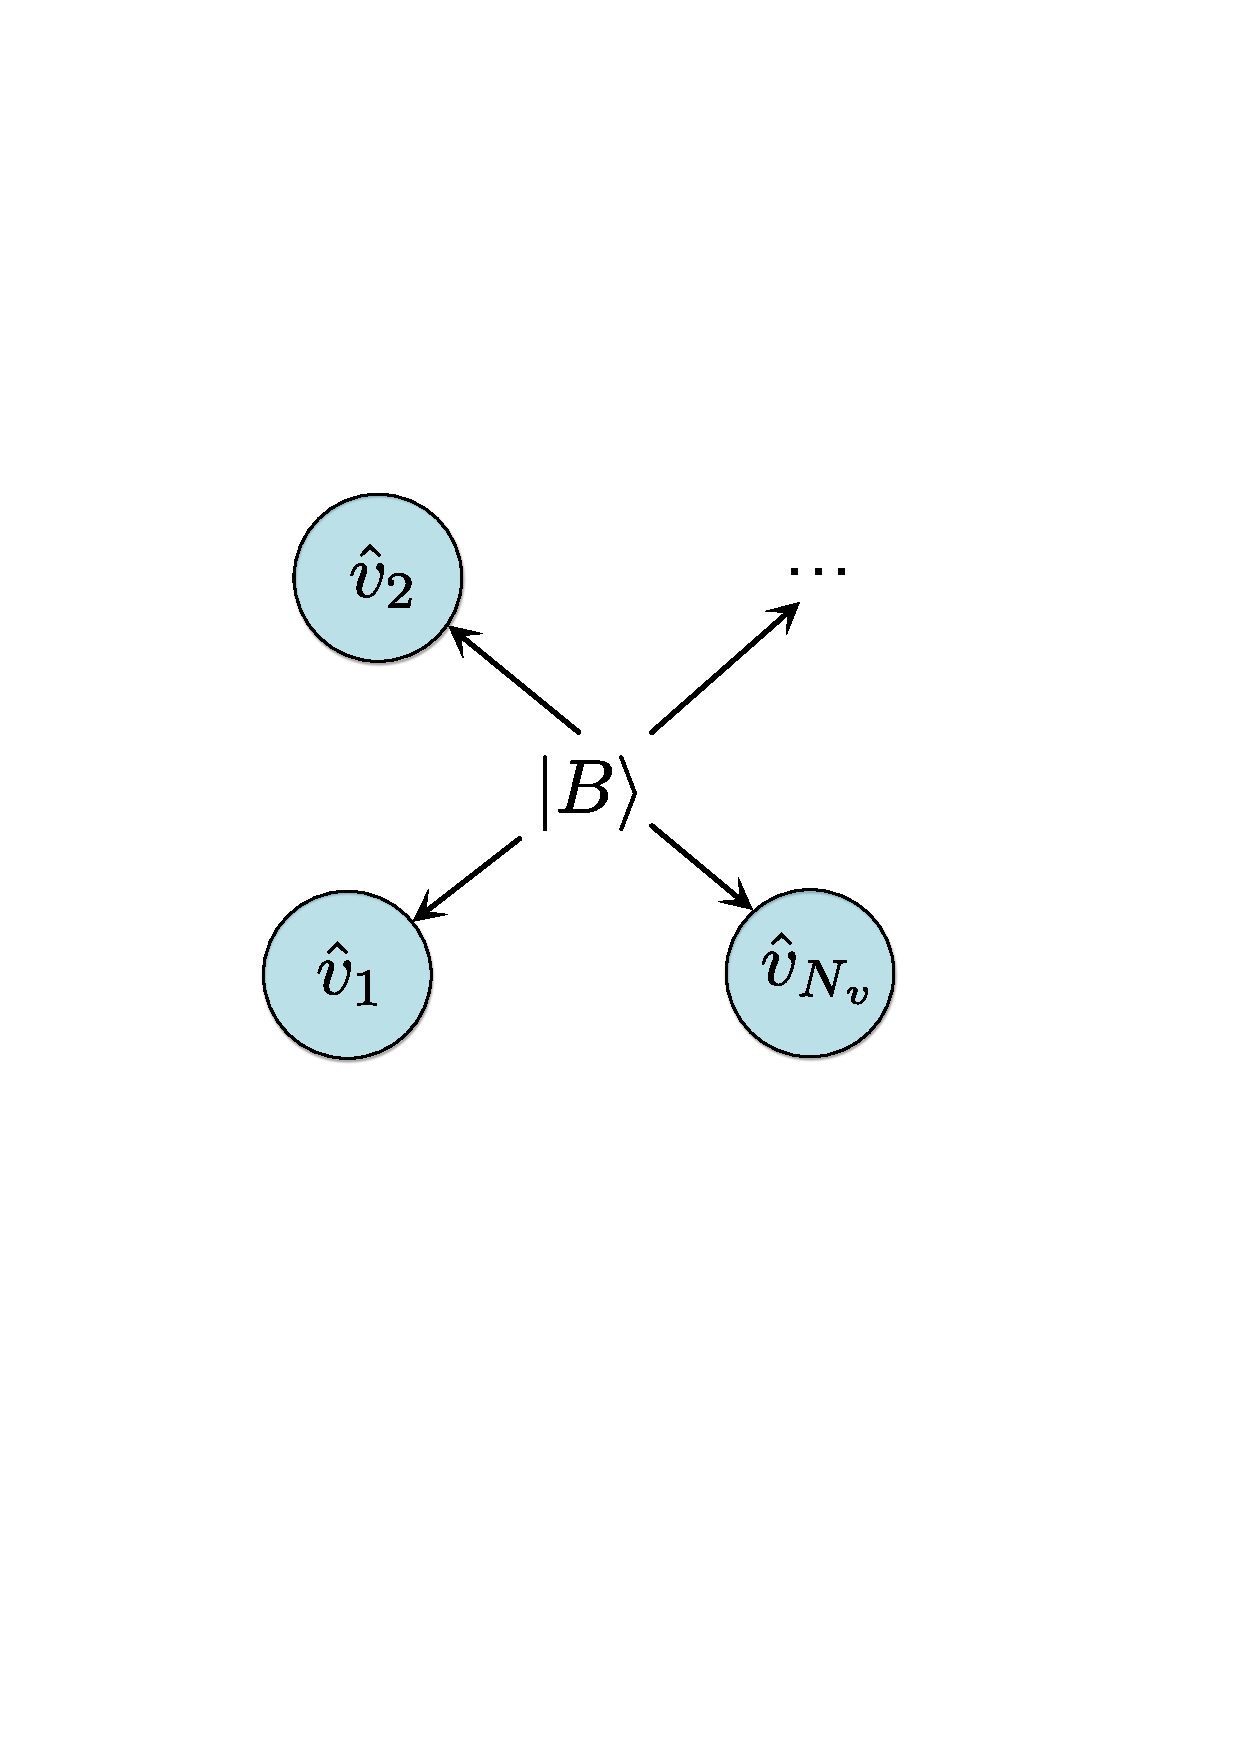
\includegraphics[width=0.6\columnwidth]{figures/quantum_voting}
\caption{Quantum anonymous voting protocol. The network distributes a bipartite \emph{ballot state} between voting booth and tallyman. All voters apply \emph{voter operators}, which encode the value of their vote into the phases in the ballot state. Following voting, the tallyman measures the joint bipartite state in an appropriate basis to recover the phase, which reflects the cumulative vote.} \label{fig:quantum_voting}
\end{figure}

\subsection{Secure quantum computation}

Until now we have focussed primarily on the security of messages. Future quantum computers are likely to be extremely expensive and owned by few. The most common model for utilising them will likely be via outsourcing them to the cloud. The types of computations performed by quantum computers are likely to be very valuable, potentially carrying important IP, trade secrets or information with national security implications. When we outsource things to the cloud today we are only protected by trust --- if the supercomputer we're outsourcing to gets hacked or is dishonest, they'll get all our important data. This raises the issue of encrypting computations as opposed to simply messages --- can a computation be outsourced such that the server executing the computation remains oblivious to the data they are processing?

\subsubsection{Homomorphic encryption} \label{homomorphic-encryption}

\emph{Homomorphic encryption} is a form of encryption whereby data is encrypted by a client and processed on a server \emph{in encrypted form}. That is, the server does not need to decrypt the data to execute computations on it, and returns the output to the client in encrypted form without knowing what it is (see Fig.~\ref{fig:QHE_model}).

\begin{figure}[!htb]
	\centering
	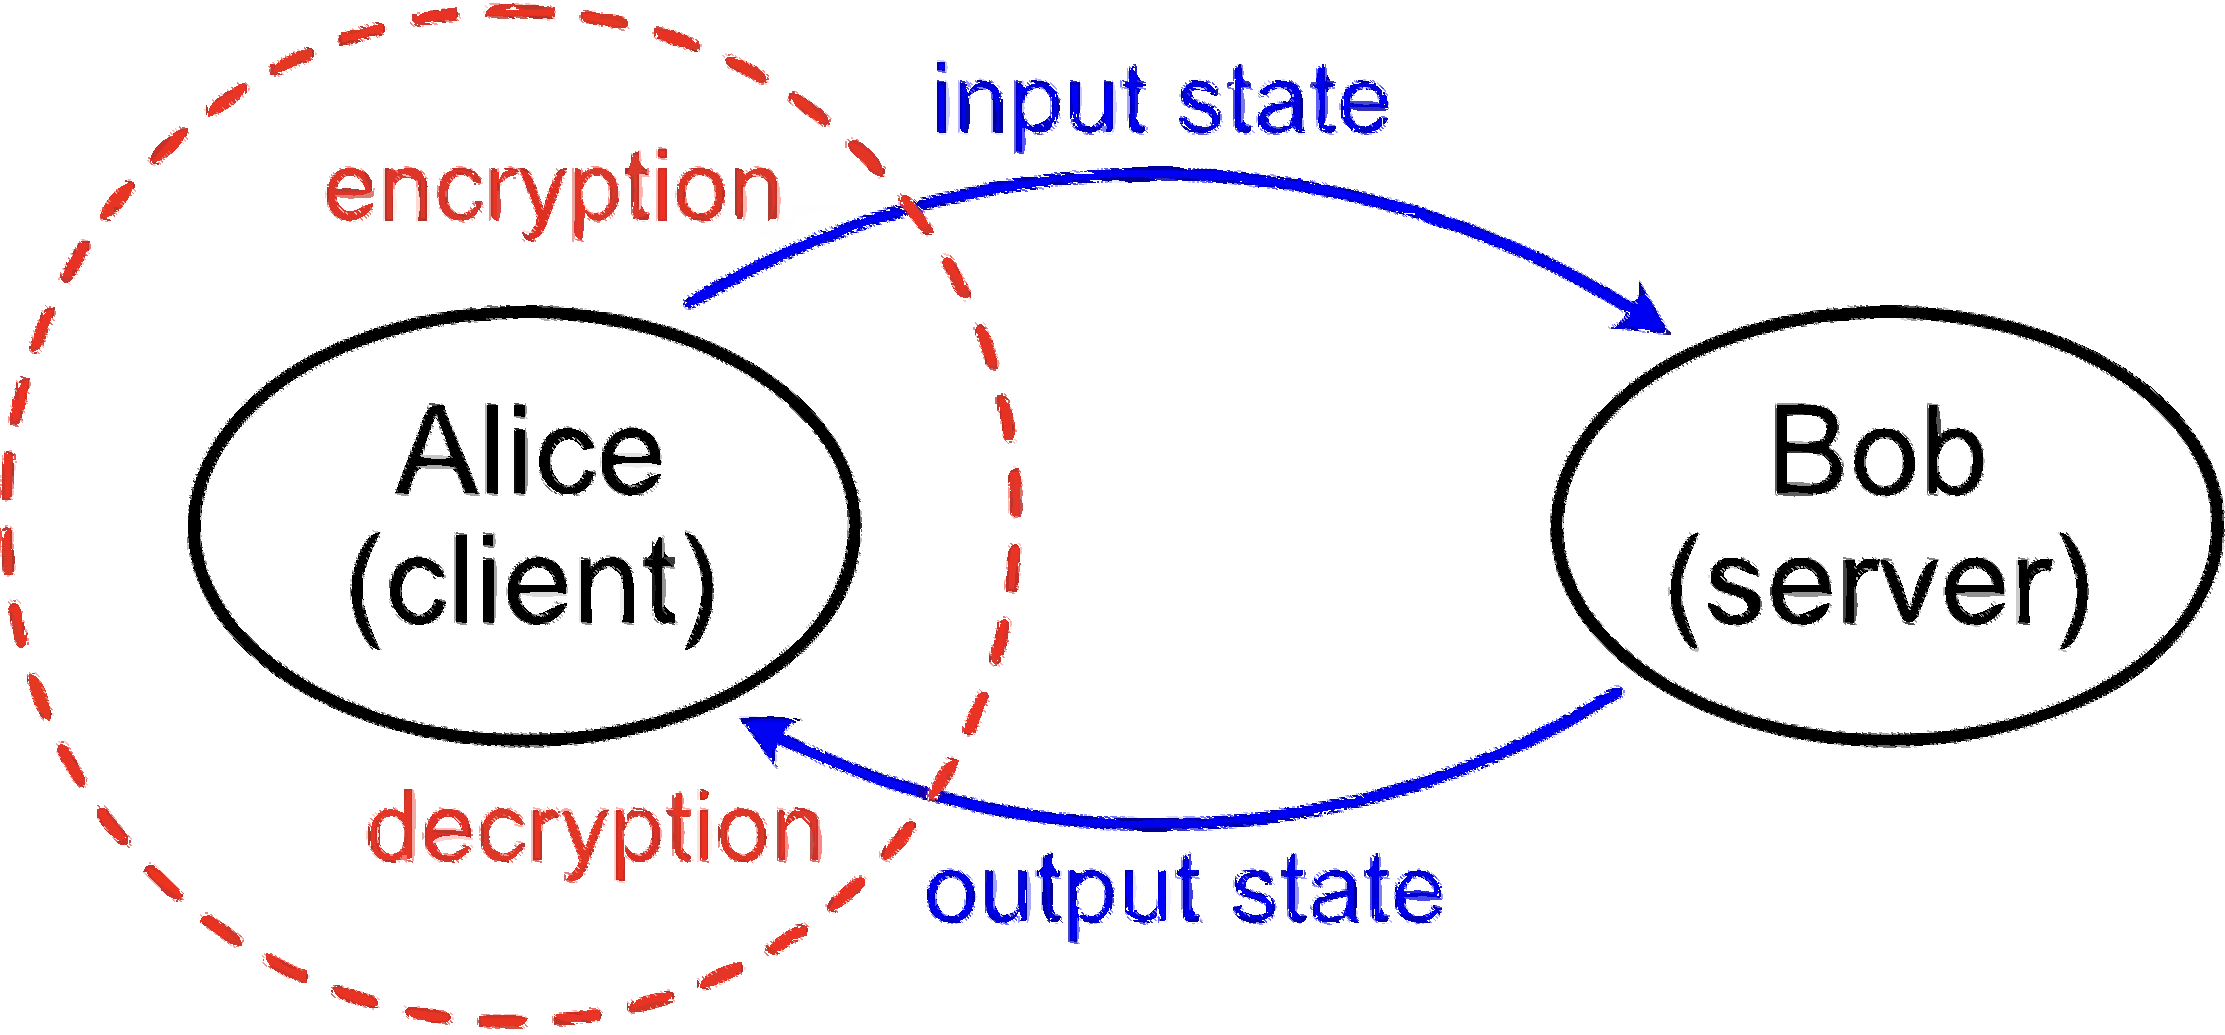
\includegraphics[width=\columnwidth]{figures/QHE}
	\caption{Quantum homomorphic encryption. Alice wishes to securely outsource a computation to Bob. Alice sends encrypted data and requires that the computation be implemented on the data in encrypted form, without first requiring decryption. The encrypted output to the computation is returned to Alice who is able to decrypt it.} \label{fig:QHE_model}
\end{figure}

Classically, homomorphic encryption is possible but highly impractical for most purposes \cite{bib:Gentry}. However, numerous approaches have been described for \emph{quantum homomorphic encryption} (QHE) \cite{bib:BJe15, bib:DSS16, bib:ouyang2020homomorphic, bib:TKOCF-qhe}. This isn't possible using only classical communication between the client and server. Instead we impose minimalistic resources for the client, comprising only state preparation, measurement and teleportation, whereas the server has arbitrary quantum resources (see Fig.~\ref{fig:outsourcing}).

\begin{figure}[!htb]
	\centering
	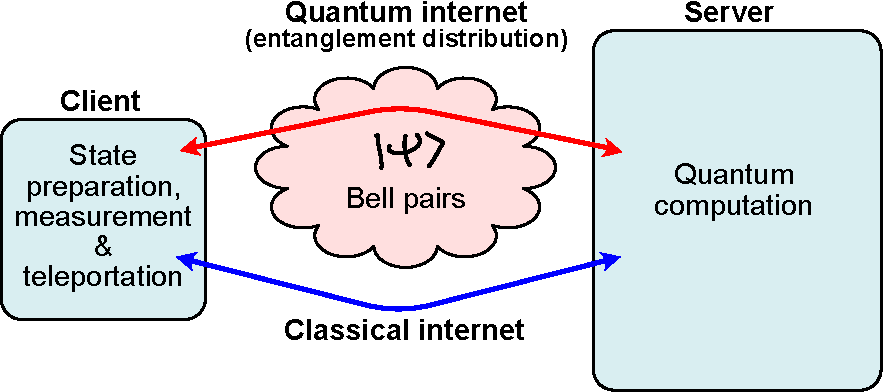
\includegraphics[width=\columnwidth]{figures/QC_outsourcing_model.pdf}
	\caption{Model for outsourced quantum computation using quantum homomorphic encryption. The client is assumed to have minimal quantum resources: state preparation, measurement and teleportation. The server has arbitrary quantum resources for large-scale quantum computation.} \label{fig:outsourcing}
\end{figure}

Perhaps the easiest to explain is QHE of Clifford circuits, which have the property that they commute with the Pauli group, satisfying,
\begin{align}
	\hat{U}_\mathrm{C} \cdot \bigotimes_{i=1}^n \hat{\sigma}_{f(i)} = \bigotimes_{i=1}^n \hat{\sigma}_{g(i)} \cdot \hat{U}_\mathrm{C},
\end{align}
where $\hat{U}_\mathrm{C}$ is a Clifford circuit, $\hat{\sigma}_i$ are the Pauli operators, and the functions $f(i)$ and $g(i)$ characterise the commutation relation between the Pauli operators and the Clifford circuit.

Suppose Alice wants to outsource her state $\hat\rho$ to the server who implements $\hat{U}_\mathrm{C}$. She encrypts it by applying one of the four Pauli operators to it, according to her key \mbox{$f(i)\in\{0,1,2,3\}$}, which is uniform and random,
\begin{align}
	\hat\rho_{\rm Alice}^{\rm enc} = \hat\sigma_{f(i)} \hat\rho_{\rm Alice} \hat\sigma_{f(i)}.
\end{align}

The server or any eavesdropper in the absence of knowing the key would observe the state,
\begin{align}
	\hat\rho_{\rm Bob}^{\rm enc} = \frac{1}{4}\sum_{k=1}^4 \hat\sigma_k \hat\rho \hat\sigma_k = \frac{\hat{I}}{4},
\end{align}
which is the completely mixed state. Since this is independent of $\hat\rho$, no information about Alice's input or output state can be known. Thus, this scheme offers information-theoretic security. Equivalently, the mutual information between Alice and Bob is identically zero,
\begin{align}
	I(A:B) = 0.	
\end{align}

Upon receiving the output, Alice can decrypt her qubits using the commuted key $g(i)$, which can be efficiently classically calculated from $f(i)$ for Clifford circuits. The model is shown in Fig.~\ref{fig:QHE_Clifford}.

\begin{figure}[!htb]
	\centering
	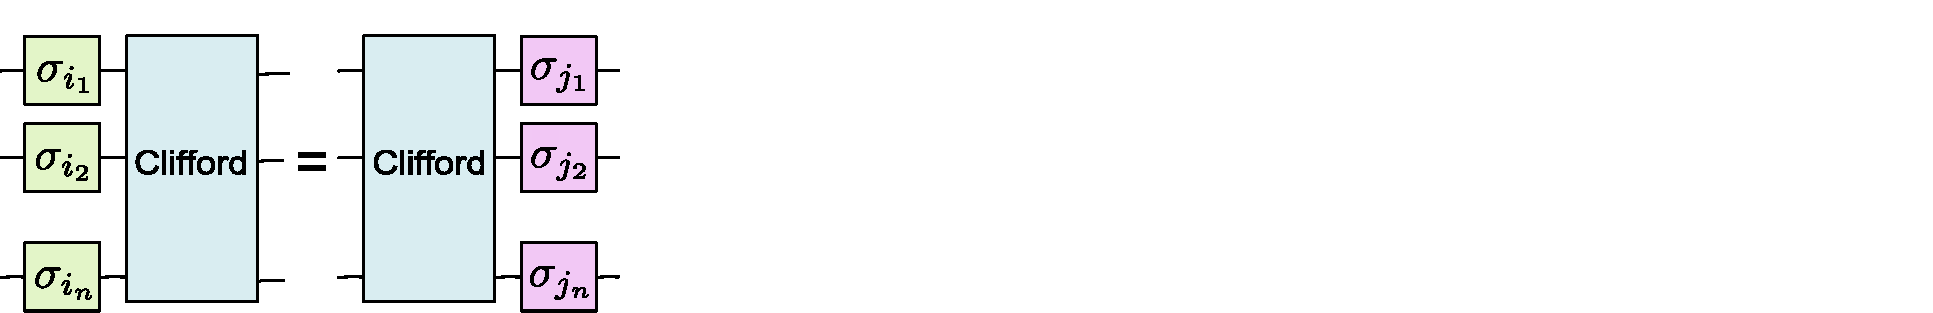
\includegraphics[width=\columnwidth]{figures/Clifford_QHE}
	\caption{Homomorphic encryption of Clifford circuits using Pauli-key encoding. This construction offers perfect information-theoretic security to Alice since the server, in the absence of knowing the key, observes a completely randomised state.} \label{fig:QHE_Clifford}
\end{figure}

The quantum computer scientists are protesting at this point that Clifford circuits are not universal for quantum computing and can be efficiently classically simulated. This is true if the input states are Clifford states, however by injecting so-called \emph{magic states} (single-qubit states of a particular form that facilitate the implementation of $T$-gates via gate teleportation), Clifford circuits can indeed be made universal for quantum computation.

A similar idea can be applied to linear optics circuits, with whom optical displacement operators, $\hat{D}(\alpha)$, commute to yield a different set of displacement operators,
\begin{align}
	\hat{U}_\mathrm{LO} \cdot \bigotimes_{i=1}^n \hat{D}_i(\alpha_i) = \bigotimes_{i=1}^n \hat{D}_i(\beta_i) \cdot \hat{U}_\mathrm{LO},
\end{align}
where $\hat{U}_\mathrm{LO}$ is a linear optics circuit comprising beamsplitters and phase-shifters, and $\hat{D}_i(\alpha_i)$ are the displacement operators on mode $i$.

The commutation relation for displacement operators acting on linear optics networks is classically efficient and obtained by simple matrix multiplication,
\begin{align}
	\vec\beta = U_\mathrm{LO}\cdot\vec\alpha.	
\end{align}

Displacement operators are easily experimentally realised using beamsplitters and coherent states produced by laser sources. This paves the way for QHE to be applied to linear optics quantum computations \cite{bib:KLM01} (see Fig.~\ref{fig:QHE_LO}).

\begin{figure}[!htb]
	\centering
	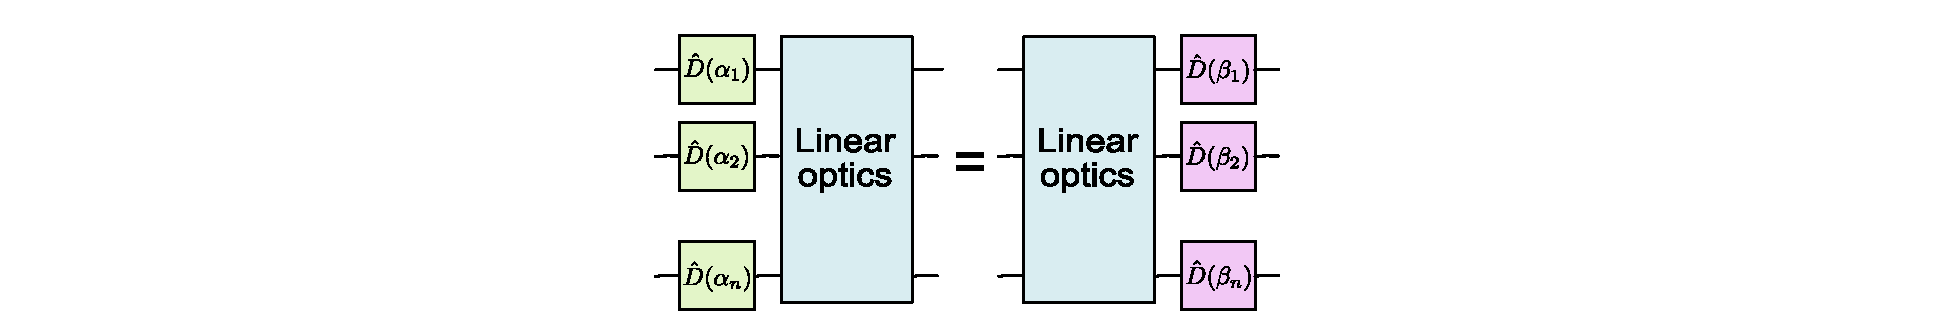
\includegraphics[width=\columnwidth]{figures/LO_QHE}
	\caption{Homomorphic encryption of linear optics circuits using displacement-key encoding.} \label{fig:QHE_LO}
\end{figure}

\subsubsection{Blind quantum computing} \label{blind-quantum-computing}

Blind quantum computing (BQC) is a stronger form of outsourced quantum computation whereby both the data \emph{and} the algorithm itself are shielded from the server \cite{bib:FitzsimonsBQC} (see Fig.~\ref{fig:blind_model}). This is particularly important for clients wishing to implement proprietary algorithms of significant value that ought to be protected. The model can be conceptualised as per the figure below.

\begin{figure}[!htb]
	\centering
	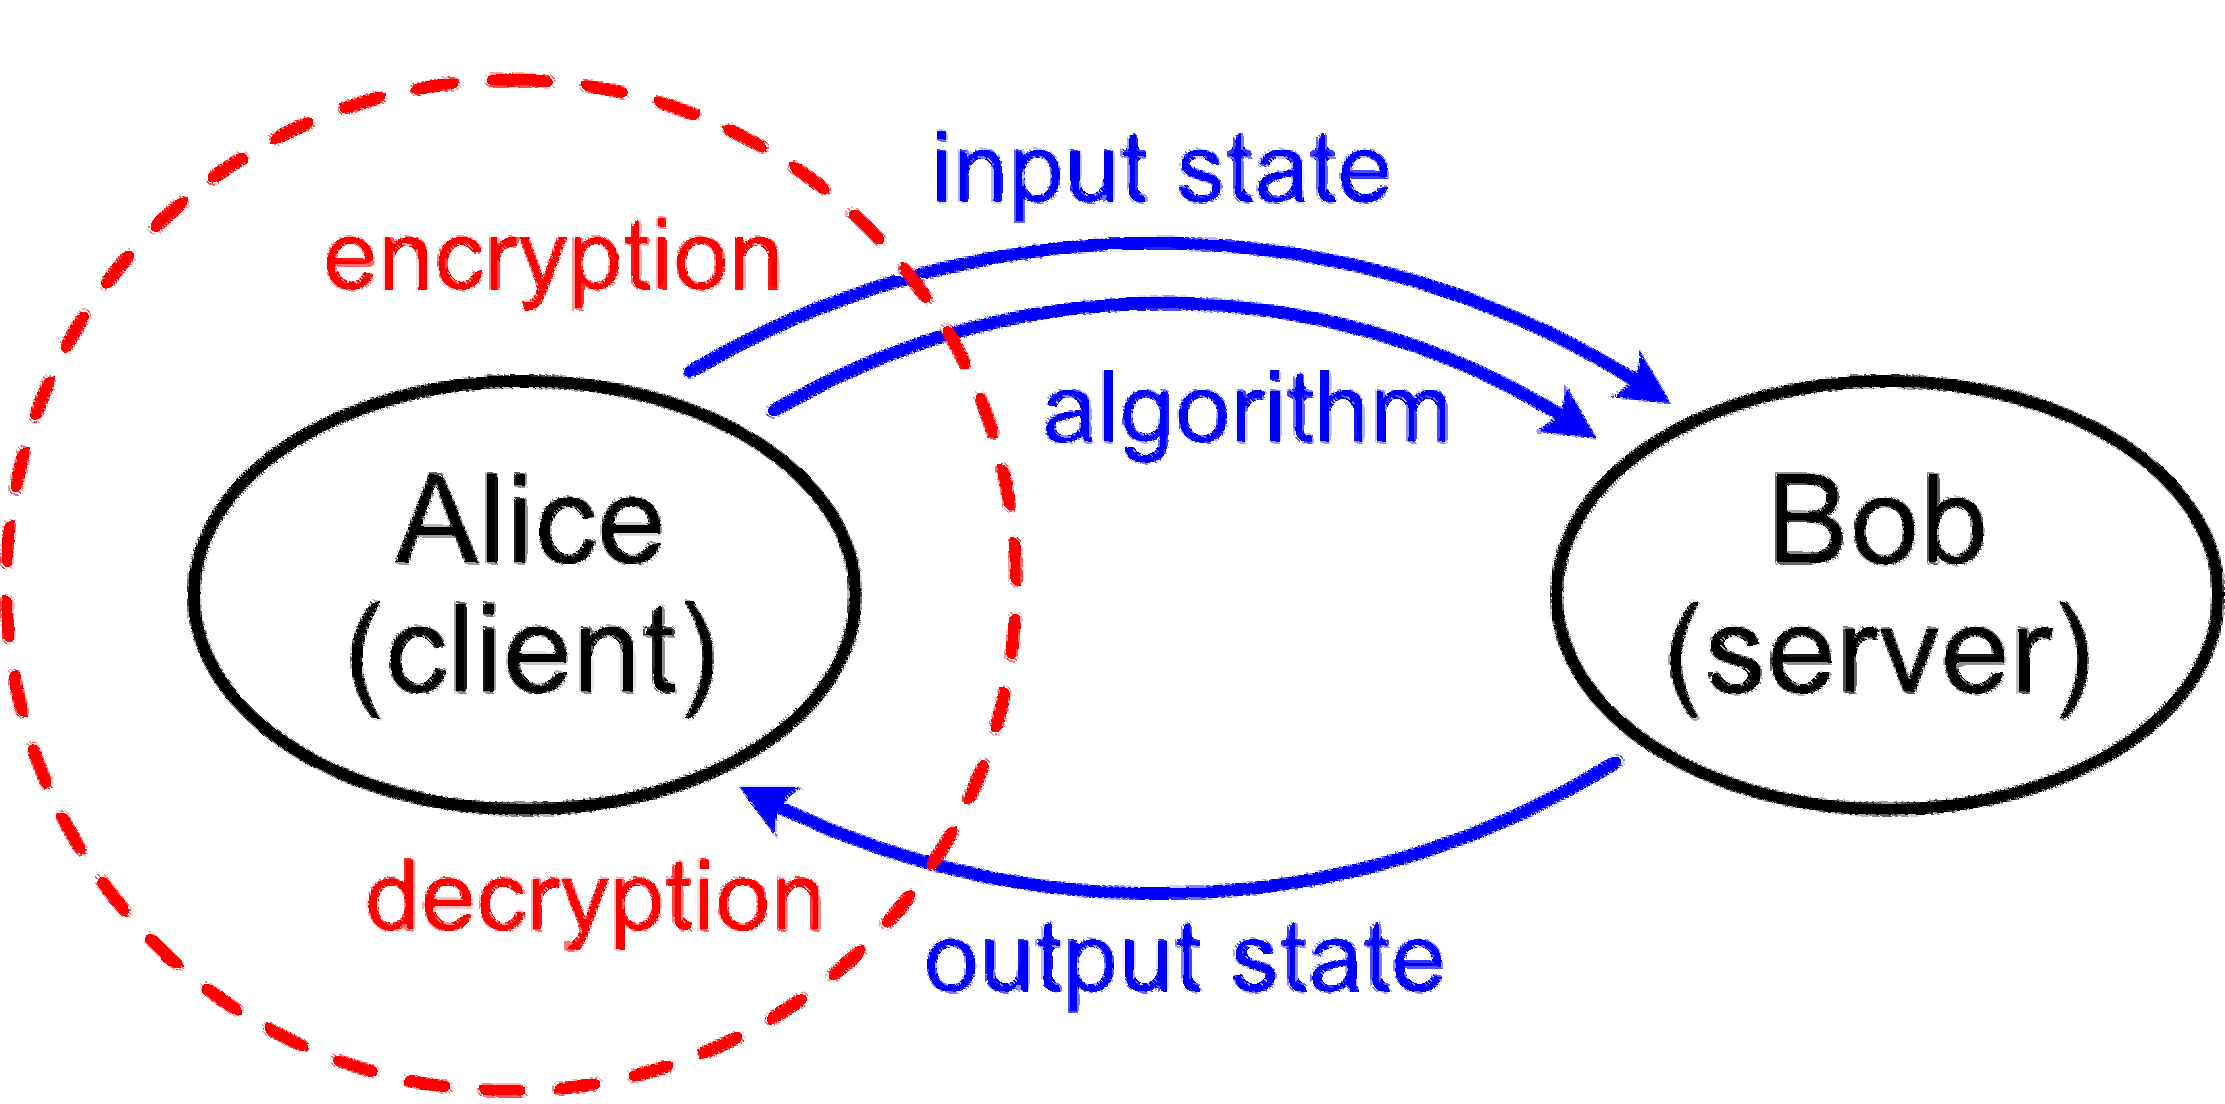
\includegraphics[width=\columnwidth]{figures/BQC}
	\caption{Blind quantum computing is similar to quantum homomorphic encryption, except that in addition to the data being encrypted, the algorithm is also. Bob is required to execute the computation without learning the algorithm or the data.} \label{fig:blind_model}
\end{figure}

While there have been many described variants for implementing blind \emph{quantum} computing, it is known that blind \emph{classical} computation is not theoretically possible.

The easiest model for BQC to describe is via the graph state model for quantum computation. Here a graph state is prepared such that vertices represent qubits and edges represent entangling controlled-phase gates. Graph states are defined only by the graph, with the remainder of the state preparation process being fixed. Formally, a graph state on graph $G=(V,E)$, where $V$ denotes vertices and $E$ denote edges, is defined as,
\begin{align}
	|G\rangle = \prod_{e\in E} \hat{\mathrm{CZ}}_e |+\rangle^{\otimes n},
\end{align}
where there are \mbox{$n=|V|$} qubits, $\hat{\mathrm{CZ}}$ is the two-qubit, maximally entangling, controlled-phase gate, and,
\begin{align}
	|+\rangle = \frac{1}{\sqrt{2}}(|0\rangle + |1\rangle).
\end{align}

Given a graph state of sufficient size, an arbitrary computation can be implemented via single-qubit measurements alone --- the so-called measurement-based model for quantum computation (MBQC) \cite{bib:Raussendorf03}. In the measurement-based model, it is the order and basis in which qubits are measured that defines the algorithm, where the order and basis choice depends upon previous measurement outcomes.

Suppose the server prepares a large graph state. Rather than perform the measurements, it communicates the qubits to the client one at a time, who performs the measurements. Now all the server knows is the graph topology, which is universal and could implement any algorithm up to a given size. This shields the server from knowing anything about the algorithm itself. The client who performs the measurements now has complete control over what algorithm is implemented (via the choice of measurements), and what the output state is (the last measured qubits). The model is shown in Fig.~\ref{fig:blind_MBQC}.

\begin{figure}[!htb]
	\centering
	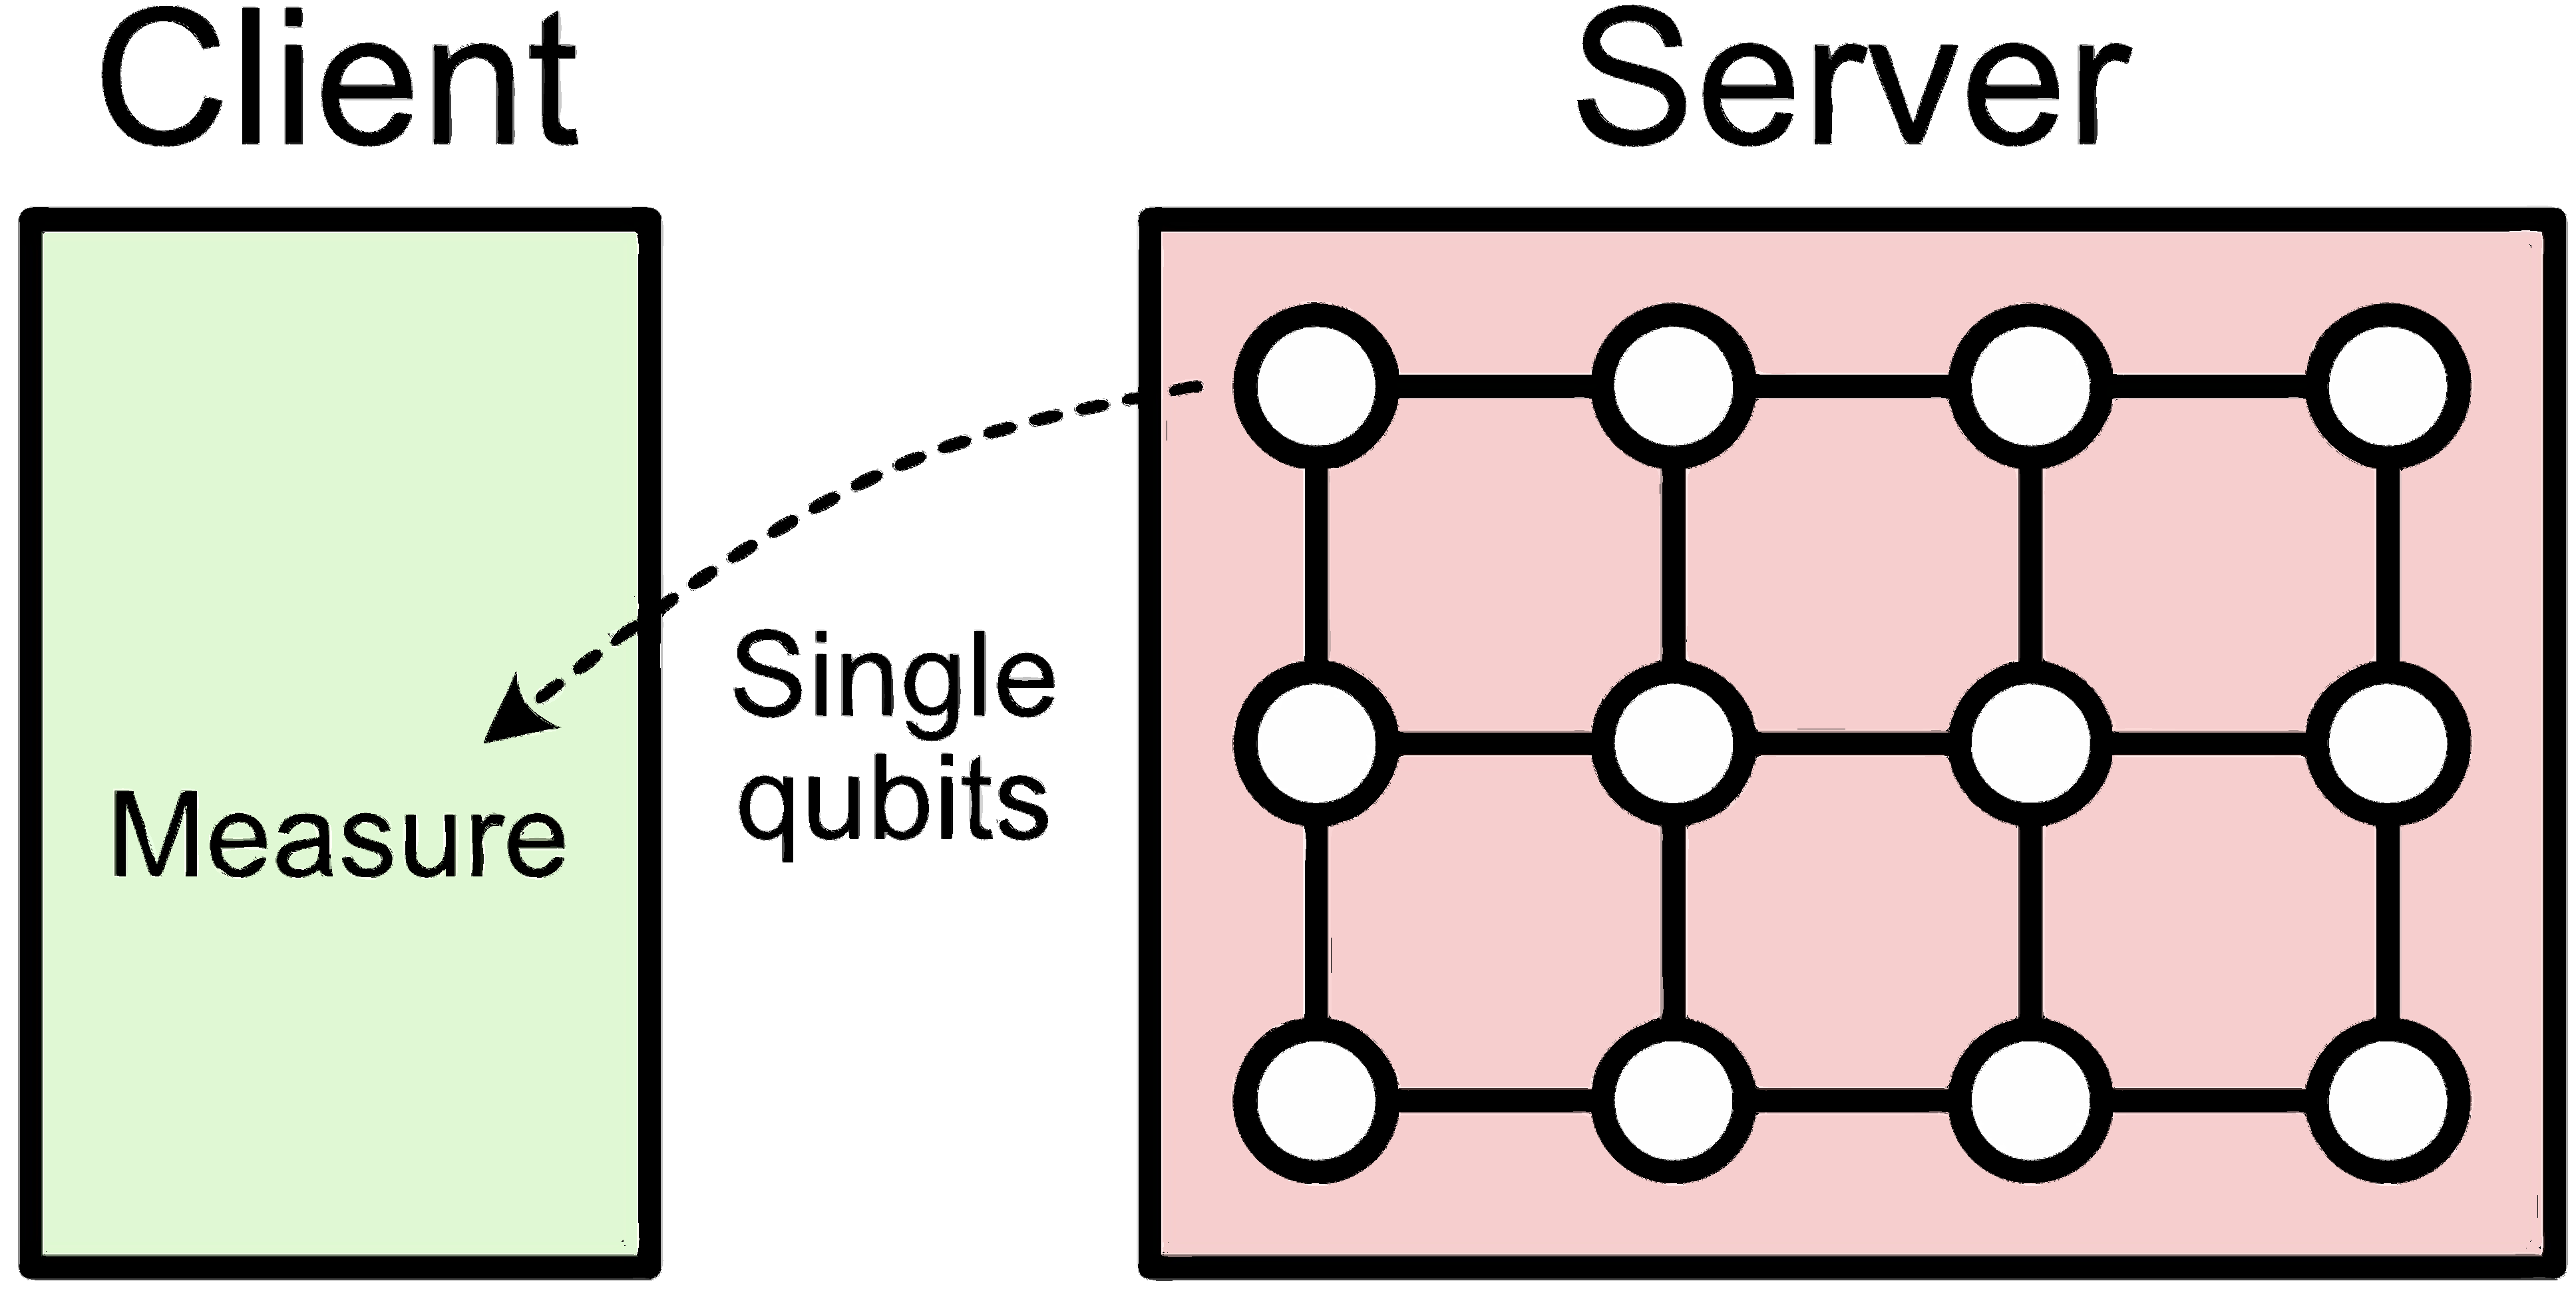
\includegraphics[width=0.75\columnwidth]{figures/BQC_MBQC}
	\caption{One of many models for blind quantum computing using the graph state model for quantum computing. The server prepares the complete graph state and communicates its qubits to the client one at a time for measurement in the appropriate basis.} \label{fig:blind_MBQC}
\end{figure}